\documentclass[12pt,]{article}
\usepackage[left=1in,top=1in,right=1in,bottom=1in]{geometry}
\newcommand*{\authorfont}{\fontfamily{phv}\selectfont}
\usepackage[]{mathpazo}

  \usepackage[T1]{fontenc}
  \usepackage[utf8]{inputenc}

\newlength{\cslhangindent}
\setlength{\cslhangindent}{1.5em}
\newenvironment{CSLReferences}[2]%
    {\setlength{\parindent}{0pt}%
    \everypar{\setlength{\hangindent}{\cslhangindent}}\ignorespaces}%
    {\par}



\usepackage{abstract}
\renewcommand{\abstractname}{}    % clear the title
\renewcommand{\absnamepos}{empty} % originally center

\renewenvironment{abstract}
 {{%
    \setlength{\leftmargin}{0mm}
    \setlength{\rightmargin}{\leftmargin}%
  }%
  \relax}
 {\endlist}

\makeatletter
\def\@maketitle{%
  \newpage
%  \null
%  \vskip 2em%
%  \begin{center}%
  \let \footnote \thanks
    {\fontsize{18}{20}\selectfont\raggedright  \setlength{\parindent}{0pt} \@title \par}%
}
%\fi
\makeatother




\setcounter{secnumdepth}{0}

\usepackage{longtable,booktabs}

\usepackage{graphicx,grffile}
\makeatletter
\def\maxwidth{\ifdim\Gin@nat@width>\linewidth\linewidth\else\Gin@nat@width\fi}
\def\maxheight{\ifdim\Gin@nat@height>\textheight\textheight\else\Gin@nat@height\fi}
\makeatother
% Scale images if necessary, so that they will not overflow the page
% margins by default, and it is still possible to overwrite the defaults
% using explicit options in \includegraphics[width, height, ...]{}
\setkeys{Gin}{width=\maxwidth,height=\maxheight,keepaspectratio}


\title{Political Donor Motivations and Public Support of Policies: A
Time-Series Analysis  }
 



\author{}


\date{}

\usepackage{titlesec}
\titleformat*{\section}{\normalsize\bfseries}
\titleformat*{\subsection}{\normalsize\itshape}
\titleformat*{\subsubsection}{\normalsize\itshape}
\titleformat*{\paragraph}{\normalsize\itshape}
\titleformat*{\subparagraph}{\normalsize\itshape}



\newtheorem{hypothesis}{Hypothesis}
\usepackage{setspace}


% set default figure placement to htbp
\makeatletter
\def\fps@figure{htbp}
\makeatother

\usepackage{graphicx}
\usepackage{booktabs}
\usepackage{longtable}
\usepackage{array}
\usepackage{multirow}
\usepackage{wrapfig}
\usepackage{float}
\usepackage{colortbl}
\usepackage{pdflscape}
\usepackage{tabu}
\usepackage{threeparttable}
\usepackage{threeparttablex}
\usepackage[normalem]{ulem}
\usepackage{makecell}
\usepackage{xcolor}

% move the hyperref stuff down here, after header-includes, to allow for - \usepackage{hyperref}

\makeatletter
\@ifpackageloaded{hyperref}{}{%
\ifxetex
  \PassOptionsToPackage{hyphens}{url}\usepackage[setpagesize=false, % page size defined by xetex
              unicode=false, % unicode breaks when used with xetex
              xetex]{hyperref}
\else
  \PassOptionsToPackage{hyphens}{url}\usepackage[draft,unicode=true]{hyperref}
\fi
}

\@ifpackageloaded{color}{
    \PassOptionsToPackage{usenames,dvipsnames}{color}
}{%
    \usepackage[usenames,dvipsnames]{color}
}
\makeatother
\hypersetup{breaklinks=true,
            bookmarks=true,
            pdfauthor={},
             pdfkeywords = {},  
            pdftitle={Political Donor Motivations and Public Support of
Policies: A Time-Series Analysis},
            colorlinks=true,
            citecolor=blue,
            urlcolor=blue,
            linkcolor=magenta,
            pdfborder={0 0 0}}
\urlstyle{same}  % don't use monospace font for urls

% Add an option for endnotes. -----


% add tightlist ----------
\providecommand{\tightlist}{%
\setlength{\itemsep}{0pt}\setlength{\parskip}{0pt}}

% add some other packages ----------

% \usepackage{multicol}
% This should regulate where figures float
% See: https://tex.stackexchange.com/questions/2275/keeping-tables-figures-close-to-where-they-are-mentioned
\usepackage[section]{placeins}


\begin{document}
% \pagenumbering{arabic}% resets `page` counter to 1 
%    

% \maketitle

{% \usefont{T1}{pnc}{m}{n}
\setlength{\parindent}{0pt}
\thispagestyle{plain}
{\fontsize{18}{20}\selectfont\raggedright 
\maketitle  % title \par  

}

{
   \vskip 13.5pt\relax \normalsize\fontsize{11}{12} 
 

}

}








\begin{abstract}

    \hbox{\vrule height .2pt width 39.14pc}

    \vskip 8.5pt % \small 

\noindent The two predominant theories of political donor motivations
are the access-oriented model and the consumption model. This paper
combines political donation records and social media posts from
politicians to examine behaviors predicted by these two theories using a
time-series methodology. The access-oriented model of donors predicts
that donations from specific groups of donors will precede public
support of certain policies. The consumption model predicts that
donations from various groups of donors will lag in response to public
support of certain policy issues. This paper statistically derives
coalitions of similar donors and tests the competing models of political
donor motivations. While post research has treated each model
monolithically, presuming that all donors operate under one model or the
other, I find evidence of both motivational models in different donors.
(Word Count: 5272)


    \hbox{\vrule height .2pt width 39.14pc}


\end{abstract}


\vskip -8.5pt


 % removetitleabstract

\noindent \doublespacing 

\newpage

\hypertarget{introduction}{%
\section{Introduction}\label{introduction}}

The amount of money raised and spent by political campaigns in the
United States continues to rise with each election cycle (Goldmacher
2020). However, the explanations of the motivations of political donors,
the psychological reasons why political donors decide to make a
contribution, remain unsettled. The predominant theories of political
donor motivation fall into two categories, the access-oriented model or
the consumption model. In the access-oriented model, contributions are
given in exchange for access to politicians (Francia et al. 2003). The
consumption model of donations sees donors as participants in the
political process who seek to alter election probabilities in a way that
helps one's preferred campaign, similar to how voting seeks to help a
campaign achieve election (Ansolabehere, Figueiredo, and Snyder 2003).
Despite taking diametric views of political donors, the two models share
the similarity that past researchers have predominantly subscribed to a
single model and don't consider the possibility of both of the models
existing in different donors. In other words, most previous scholarship
on political donors does not allow for the possibility that different
political donors may have differing reasons for making their
contribution.

The present work eschews this zero-sum view of the motivations of
political donors. Instead, the two predominant models are both
investigated under assumptions that allow them to co-exist by looking
for both motivational models among different groups of donors.
Researchers readily operate under the idea that individuals can have
differing reasons for why and how they vote (e.g. Arceneaux and
Nickerson 2009; Feldman 1982; Lau 1985; Rahn, Krosnick, and Breuning
1994; Yiannakis 1981). Then why has so much of past research on donors
either pitted the two models of donor motivations against one another
(e.g. Welch 1980) or operated exclusively in the domain of either the
access-oriented model (e.g. Baker 2020; Fellowes and Wolf 2004;
Fouirnaies and Hall 2015; Francia, Green, Herrnson, Powell, and Clyde
Wilcox 2003; Herndon 1982; Kalla and Broockman 2016; Langbein 1986;
Powell and Grimmer 2016) or consumption model (e.g. Ansolabehere,
Figueiredo, and Snyder 2003)?

This paper makes three main contributions to the literature on political
donors. First, it tests the two models of political donors in a way that
allows both models to exist among different donors. Second, instead of
arbitrary classification of donors, such as large versus small donors, I
take a bottom-up network approach to studying political donors where
donors are clustered together based on network connections based on
donations patterns. Finally, I layer in social media data to fundraising
data and show the value that using politicians' social media data can
have on understanding political actors. Using these novel approaches to
understanding political donor behavior, we find evidence that both
models, the access-oriented and consumption models, likely exist, but
within different donors.

\hypertarget{access-oriented-model}{%
\section{Access-Oriented Model}\label{access-oriented-model}}

Access-oriented political donors attempt to use their contributions to
gain access to politicians. Most often, access-oriented motivations are
thought to be the reason behind contributions from large donors. The
idea is that donations can gain individuals access to politicians and
their staff to influence legislative behaviors (Francia, Green,
Herrnson, Powell, and Clyde Wilcox 2003).

Congress is an information ecology where competing facts and
perspectives are everywhere and ever-changing. Providing political
contributions can allow political contributors to gain direct access by
cutting through all the noise of competing information that the
legislator might be encountering (Milbrath 1958). Interest groups and
individuals hope to gain access to politicians through their financial
contributions in order to influence government policies (Baker 2020;
Fouirnaies and Hall 2015; Herndon 1982; Powell and Grimmer 2016). These
attempts to buy access are successful in gaining meetings with
congressional offices for both special interest groups (Langbein 1986)
and individual donors (Kalla and Broockman 2016).

Contributions from financial (Hayes 2017), telecommunications (Edwards
and Figueiredo 2016), education (Constant 2006), environmental (Hogan
2020) and healthcare interest groups (McKay 2018) have all influenced
legislation. Whatever connection does exist between campaign
contributors and public policy has a stronger impact if the
contributions are from organized business interests within a member's
district (Hall and Wayman 1990). While it is ``nearly universal''
(Bonica 2016) that corporate executives of Fortune 500 firms make
political contributions (Fremeth, Richter, and Schaufele 2013), there is
heterogeneity in their political leanings (Bonica 2016).

Potentially, the influence exerted by contributors when making a
contribution is so indirect that it does not always materialize in
statistical patterns of legislative voting or public policy. Yet there
is evidence of the influence towards the benefit of the financial
contributor. Firms that contribute to winning political campaigns have
abnormal financial returns after the election (Akey 2015; Cooper, Gulen,
and Ovtchinnikov 2010x). In addition to immediately-felt financial
returns, donors may systematically contribute money to legislative
agenda setters, such as chairs of financial committees, in an effort to
set future legislative agendas (Fouirnaies and Hall 2018). Even business
executives understand that political contributions are purchases of
``good will'' which are positive in return but are not frequent nor
universal (Gordon, Hafer, and Landa 2007). For example, political
contributions reduce the punishment for business executives who are
sanctioned for committing fraud (Fulmer, Knill, and Yu 2017); increase
the number of ``sweetheart'' contracts awarded from the government
(Ferris, Houston, and Javakhadze 2019); and increase the premium and
survivability of Initial Public Offerings (IPOs) (Gounopoulos, Mazouz,
and Wood 2021).

As this review makes clear, most of the existing work examines the
effect of donations on legislative behaviors. However, this paper
instead examines a similar but distinct topic: whether political
donations impact position-taking by politicians. The literature in this
area is far more sparse, and so my hypotheses are guided by the body of
research on legislative behavior.

Specifically, I focus on how the timing of political donations reveals
information about donor motivations. Under the access-oriented model of
political donor motivations, one would expect to find politicians to be
more supportive of certain policy issues after receiving campaign
contributions from access-oriented donors. This hypothesis will be
tested using a Granger causality model (Granger 1969), which is an
econometric methodology to test whether changes in one time series
predict future changes in another time series.

\textbf{\(H_{1a}\): Donations from coalitions of political donors will
precede, or Granger cause, increased public support of certain political
issues from the politicians to whom they donate.}

Since access-oriented donors are thought to be wealthier contributors,
sometimes seeking access for financial gain, this paper will also
examine the amount contributed by members of donor coalitions that are
accepted by \(H_{1a}\).

\textbf{\(H_{2a}\): Donors from access-oriented coalitions will on
average be \emph{larger} contributors to political campaigns than donors
not in access-oriented coalitions.}

\hypertarget{consumption-model}{%
\section{Consumption Model}\label{consumption-model}}

While the access-oriented model is centered on donors \emph{influencing}
the political process, the consumption model is about donors
\emph{participating} in the political process. The consumption model of
political donors concludes that political contributions are not vehicles
by which donors seek access to politicians but instead are acts of
consumption, or in other words, participation (Ansolabehere, Figueiredo,
and Snyder 2003). Under this model, individual donors are intrinsically
motivated by ideology (Ansolabehere, Figueiredo, and Snyder 2003).
People do not receive a direct benefit by making a political donation,
but they do experience the indirect benefits of participating in a
political campaign that matches their ideology. Put otherwise, for
consumption-motivated donors, making a contribution is just an extension
of voting on a participatory spectrum. Under this approach, donations
are a way for individuals to participate and be responsive to their
``perception of the stakes in the election'' (Hill and Huber 2017).

Ideological proximity, or the spatial distance between the ideology of
candidates and donors, is an important component to the consumption
model of political donors, (Ensley 2009). It is potentially of greater
importance than agreement between the donor and the candidate on
specific policy issue positions (Barber, Canes-Wrone, and Thrower 2019),
such as taxes, global warming, and gay rights. Studies have shown that
the similarity between a donor's policy preferences and a senator's
roll-call votes is a predictor of whether a donor makes a contribution
(Barber, Canes-Wrone, and Thrower 2017). However, it is unclear if this
connection between contributors' policy preferences and legislators'
votes holds historically or only recently (Canes-Wrone and Gibson 2019).
Divergence of ideology among the candidates for an office, such as a
more extreme political opponent, does not impact donors' decisions to
make a contribution (Ensley 2009). The theoretical implications for this
paper are that consumption-oriented donors will contribute to
politicians who already show support for the policy issues, or are
ideologically proximate, to themselves. In other words, donors reward
for policy proximity between themselves and candidates.

Altogether, under the consumption model of donor motivations one would
expect public support of policy issues to attract political donors who
care about that policy, which leads to \(H_{3}\).

\textbf{\(H_{1b}\): Public support from politicians on certain political
issues will precede, or Granger cause, donations from coalitions of
political donors.}

Individual donors, as opposed to PACs, continue to make up a clear
majority of donations to political candidates (Heerwig 2016). These
individual donors most often exhibit behavior consistent with the
consumption model of donations (Barber 2016; Heerwig 2016). Further,
individual donors arguably play an even more central role in politics
more recently with the growth in small-dollar individual donors.

With the rise of small-dollar donors on the internet and the assumption
that these donors fit under the consumption model of donor motivations,
this paper will examine the amount of money contributed by members of
donor coalitions that are accepted by \(H_{1b}\).

\textbf{\(H_{2b}\): Donors from consumption coalitions will on average
be \emph{smaller} contributors to political campaigns than donors not in
consumption coalitions.}

\hypertarget{rise-of-small-dollar-donors}{%
\section{Rise of Small-Dollar
Donors}\label{rise-of-small-dollar-donors}}

The growing number of small-dollar donors in the political process
suggests that there will be more consumption-oriented donors in the
future. The anecdotal examples of the Bernie Sanders and Donald Trump
2016 and 2020 presidential campaigns, both of which received a large
number of small-dollar donors (Choma and Voght 2020), illustrate the
consumption-oriented model's connection to such donors. Small-dollar
donors likely did not directly access or influence the politics of the
Sanders or Trump campaigns. Instead, donors reacted to their messages
and decided to move further down the participatory spectrum in those
campaigns. Individual contributors are mostly participants in politics
without an ulterior motive. They are ``fickle financiers of elections''
whose donation habits can be disrupted by little changes to their worlds
such as moving to an area that is more or less Democratic or Republican
(Kettler and Lyons 2019).

The Democratic Party as a whole has expanded the proportion of its
funding that comes from small-dollar donors (Albert and Raja 2020).
Moreover, incumbents have been able to sustain their small-dollar
fundraising programs (Heberlig and Larson 2020)--suggesting that this
trend is not going to go away. This growth in small-dollar donors has
created a donorate that is more demographically representative of
America but is more ideologically extreme (Albert and Raja 2020) and one
that gives indiscriminately to incumbents, challengers, and open seat
candidates (Culberson, McDonald, and Robbins 2019). It is conceivable
that campaigns that rely on small donors will adopt rhetoric and tout
their ``outsider'' status in an effort to activate these small, more
ideologically extreme donors (Arbour 2020). For instance, extremist
politicians can leverage polarizing events to raise more money for their
campaigns (Oklobdzija 2017). As a result, some have predicted that
small-dollar donors will polarize the nation's politics even further
(Oklobdzija 2017). Although legislators who receive a large proportion
of their funds from small-dollar donors are not more polarized in their
legislative votes when they take up a more polarized agenda, they
attract an increased number of small-dollar donors in the subsequent
election (Keena and Knight-Finley 2019). This provides further evidence
for the consumption model of political donor motivations. Other studies
have agreed that mass donors are the cause of partisan polarization
(Raja and Wiltse 2012), but this conclusion is not definitive (Harden
and Kirkland 2016). Therefore, even though small-dollar donors
themselves may not be polarizing, they may provide incentive for
politicians to take more polarized positions.

This research paper will also examine the polarization of political
donor coalitions and whether consumption-oriented donors and
access-oriented donors are in polarized positions in the donor network
graph.

\textbf{\(H_{3a}\): Consumption-motivated donors will be more polarized
in the political donor network than non-consumption donors.}

\textbf{\(H_{3b}\): Access-oriented donors will be less polarized in the
political donor network than non-access donors.}

\hypertarget{data}{%
\section{Data}\label{data}}

Data for this research come from two primary sources: politicians'
social media posts and data on political donation data.

For social media posts, this paper used the Facebook (Barbera, Geisler,
and Atteveldt 2017) and Twitter (Kearney 2019) APIs to collect social
media posts from all candidates for the Wisconsin State Senate and
Wisconsin State Assembly during the 2016 election cycle (\emph{n} =
82,851). A random subset of 12,364 posts, or about 15\% of the total
posts collected, were hand-coded into 27 topical categories. These
topical categories included if the post was made in support or
opposition to a policy. For example, the ``voting liberal'' category
contains posts that are supportive of repealing voting ID laws and
expanding early voting whereas the ``voting conservative'' category
contains posts that are in support of voter ID laws and other
conservative voting reforms.

These posts were used to train and test a BERT deep learning transfer
model where about 90\% (or 11,128) were used in the training set and
about 10\% (or 1,236), were used in the test set. This trained model
achieved 82.9\% accuracy in categorizing the topic of posts in the
held-out test set. Furthermore, this model was applied to the rest of
the uncoded corpus that were later used for aggregations and
calculations of the topics that politicians were posting about.

BERT, which stands for Bidirectional Encoder Representations from
Transformers, is a pre-trained deep learning model to which researchers
can add additional output layers, in this case to classify social media
posts into the hand-coded topical categories (Devlin et al. 2019). BERT
is currently a state-of-the-art model in the field of Natural Language
Processing (Devlin, Chang, Lee, and Toutanova 2019). BERT and other
transfer learning models have yet to be widely adopted by political
scientists but are an ideal choice for political science text
classification, especially when compared to traditional text-as-data
methods in the discipline (Terechshenko et al. 2020). BERT has been
applied to other social media research such as the detection of
propaganda (Vlad et al. 2019), misinformation (Jiang et al. 2020), hate
speech (Mozafari, Farahbakhsh, and Crespi 2020), stance (Tian et al.
2020), and aggression (Ramiandrisoa and Mothe 2020).

Social media can be useful in studying politics because digital
communication methods are similar to traditional political communication
and can be extrapolated to offline characteristics. The differences that
are seen in online political communication, such as lowered costs and
eased barriers to entry, represent a ``difference-of-degree'' and not a
paradigm shifting ``difference-in-kind'' (Karpf 2010). There is a strong
connection between online channels of communication in the form of
social networks and offline connections, including the building and
maintenance of social capital from those offline connections (Cranshaw
et al. 2010; Ellison and Steinfield 2006; Liben-Nowell et al. 2005;
Scellato et al. 2010). Online social networks have also been used to
study offline-based actions and beliefs like opinion polarization (Lee
et al. 2014), political polarization (Hanna et al. 2013), political
participation (Lawrence, Sides, and Farrell 2010) and political
discourse (Kushin and Kitchener 2009). Contemporary campaigns discuss
similar topics across campaign media, including social media (Kang et
al. 2018), meaning that few topic would be exclusive to, or exclusive
from, social media.

Individual political donation data for all candidates to the Wisconsin
State Legislature during the 2016 election cycle were collected from the
Wisconsin Campaign Information System (CFIS). Anonymous contributions
were removed, names were made uniform (removed punctuation, made all
names lowercase, etc.), and OpenRefine (Ham 2013) was used to stem names
to identify people who might be the same person (e.g., Jim Smith and
James Smith). To ensure that people who have the same name, but are
different people, were not counted as the same individual, their zip
code was appended to the end of their name to create a unique
identifier. Finally, only contributions from donors who contributed to
more than one campaign were used, following previous research that
emphasizes the importance of repeat donors, particularly when making
inferences (Heerwig 2018). These steps left 28,858 donations from 7,567
donors.

These donations were used to create a network of political donations
with candidates and donors serving as nodes and donations between them
as edges. This network was clustered into 13 distinct communities so
that donors in each community are most similar to one another based on
which campaigns they contributed to. The Louvain method as implemented
by Gephi (Bastian, Heymann, and Jacomy 2009) did the clustering, or
community detection.

This donor cluster network is visualized in Figure 1 using the Yifan Hu
layout algorithm (Hu 2005) with the two political parties clearly
divided with two large groups of donors, Democrats on the left, and
Republicans on the right. The graph is colored by the statistical
community the donor and candidates are in.

\begin{figure}
\centering
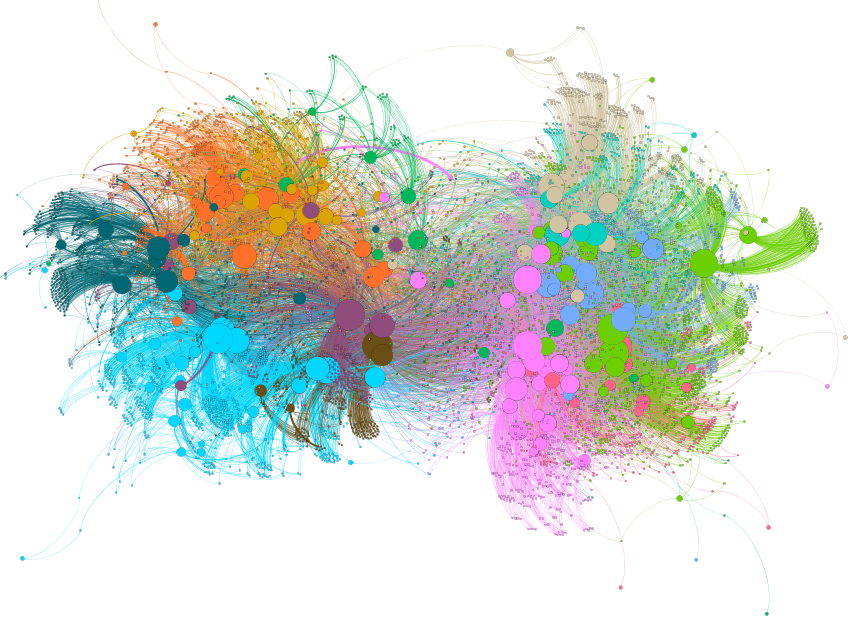
\includegraphics{../tables_and_figures/fig_1_white.png}
\caption{Network of political donors in Wisconsin in 2016. Each node
(dot) is a donor or a campaign. Each edge (line connecting two nodes)
represents a contribution. Nodes are sized by their in-degree, the
number of contributions the node received. Nodes are colored by their
assigned statistical cluster. The large bunch on the left are Democrats.
The other large group on the right are Republicans.}
\end{figure}

\hypertarget{results}{%
\section{Results}\label{results}}

\hypertarget{donor-motivation-models}{%
\subsection{Donor Motivation Models}\label{donor-motivation-models}}

\(H_{1a}\) and \(H_{1b}\) test the relationships between the social
media dataset and the political donation dataset. I tested the two
models of political donor motivations using a Granger causality
time-series model. Other social media studies have used this methodology
(Freelon, McIlwain, and Clark 2018; Lukito 2020). For example, other
researchers have used it to study the relationship between social media
and non-social media events such as offline protests (Bastos, Mercea,
and Charpentier 2015) and stock prices (Park, Leung, and Ma 2017).
Granger causality detects whether movements in one time series precedes,
lags, has a confounding variable, or is not related to another time
series (Granger 1969). An abbreviated version of this methodology takes
two time series variables X and Y. First, one builds a vector
autoregression (VAR) model to predict the outcome variable Y with Y
being the sole predictor in the model. In other words, the model only
uses Y to predict Y. Then, a second model is built where both variables
X and Y are used to build the VAR to predict Y. Effectively, if the
second model, with the inclusion of X, does a better job of predicting Y
than the first model alone, as measured by an \emph{F}-statistic, X is
said to Granger cause Y. To test for the possibility of counfounding
variables, the methodology flips X and Y and performs the same process.
If the null is rejected in both instances, then there is likely a
confounding variable Z. This analysis was conducted in R (R Core Team
2013) with the \texttt{lmtest} package (Zeileis and Hothorn 2002).
P-values were adjusted with the Bonferroni method (Haynes 2013). The
optimal lag for each model was calculated using a Bayesian Information
Criteria (Ahelegbey, Billio, and Casarin 2016) implemented by the
\texttt{tsDyn} package (Stigler 2010). Altogether, this method allows me
to test whether politicians' social media posts and donations from
groups of donors are likely related.

I compare two time series, one of social media posts and another of
political contributions from clusters of donors. The first time series
constists of the number of social media posts per day for each topic
that were made by campaigns. The analysis only included campaigns that
received contributions from a donor cluster. In other words, a time
series of donations from a donor coalition was compared to the aggregate
count of posts about a given topic made by candidates that the donor
cluster contributed to. For example, donations from donor coalition 6
Granger caused politicians that received donations from the coalition to
publicly support women's issue and pro-choice policies. Stated another
way, donations from coalition 6 predict whether candidates will publicly
support pro-women policies. The theoretical connection to political
donor psychology is that this behavior is expected under the
access-oriented model of political donor motivations. Coalitions and
policy topics that are accepted by either \(H_{1a}\) or \(H_{1b}\) are
in Table 1. The full results of the Granger causality tests are
visualized in Figure 2.

\begin{longtable}[]{@{}rllrrl@{}}
\caption{H1a and H1b acceptances}\tabularnewline
\toprule
coalition & policy topic & model & Lag & F-statistic & p-value \\
\midrule
\endfirsthead
\toprule
coalition & policy topic & model & Lag & F-statistic & p-value \\
\midrule
\endhead
0 & veterans issues: bipartisan & consumption & 5 & 7.6 &
\textless.001 \\
1 & veterans issues: bipartisan & access & 7 & 7.1 & \textless.001 \\
1 & drug abuse: bipartisan & consumption & 7 & 4.5 & \textless.001 \\
3 & race issues: liberal & access & 4 & 6.7 & \textless.001 \\
4 & guns: conservative & consumption & 4 & 6.5 & \textless.001 \\
6 & abortion and women's issues: conservative & access & 2 & 14.2 &
\textless.001 \\
7 & drug abuse: bipartisan & consumption & 7 & 5.7 & \textless.001 \\
11 & infrastructure: liberal & consumption & 7 & 5.8 & \textless.001 \\
\bottomrule
\end{longtable}

\begin{figure}
\centering
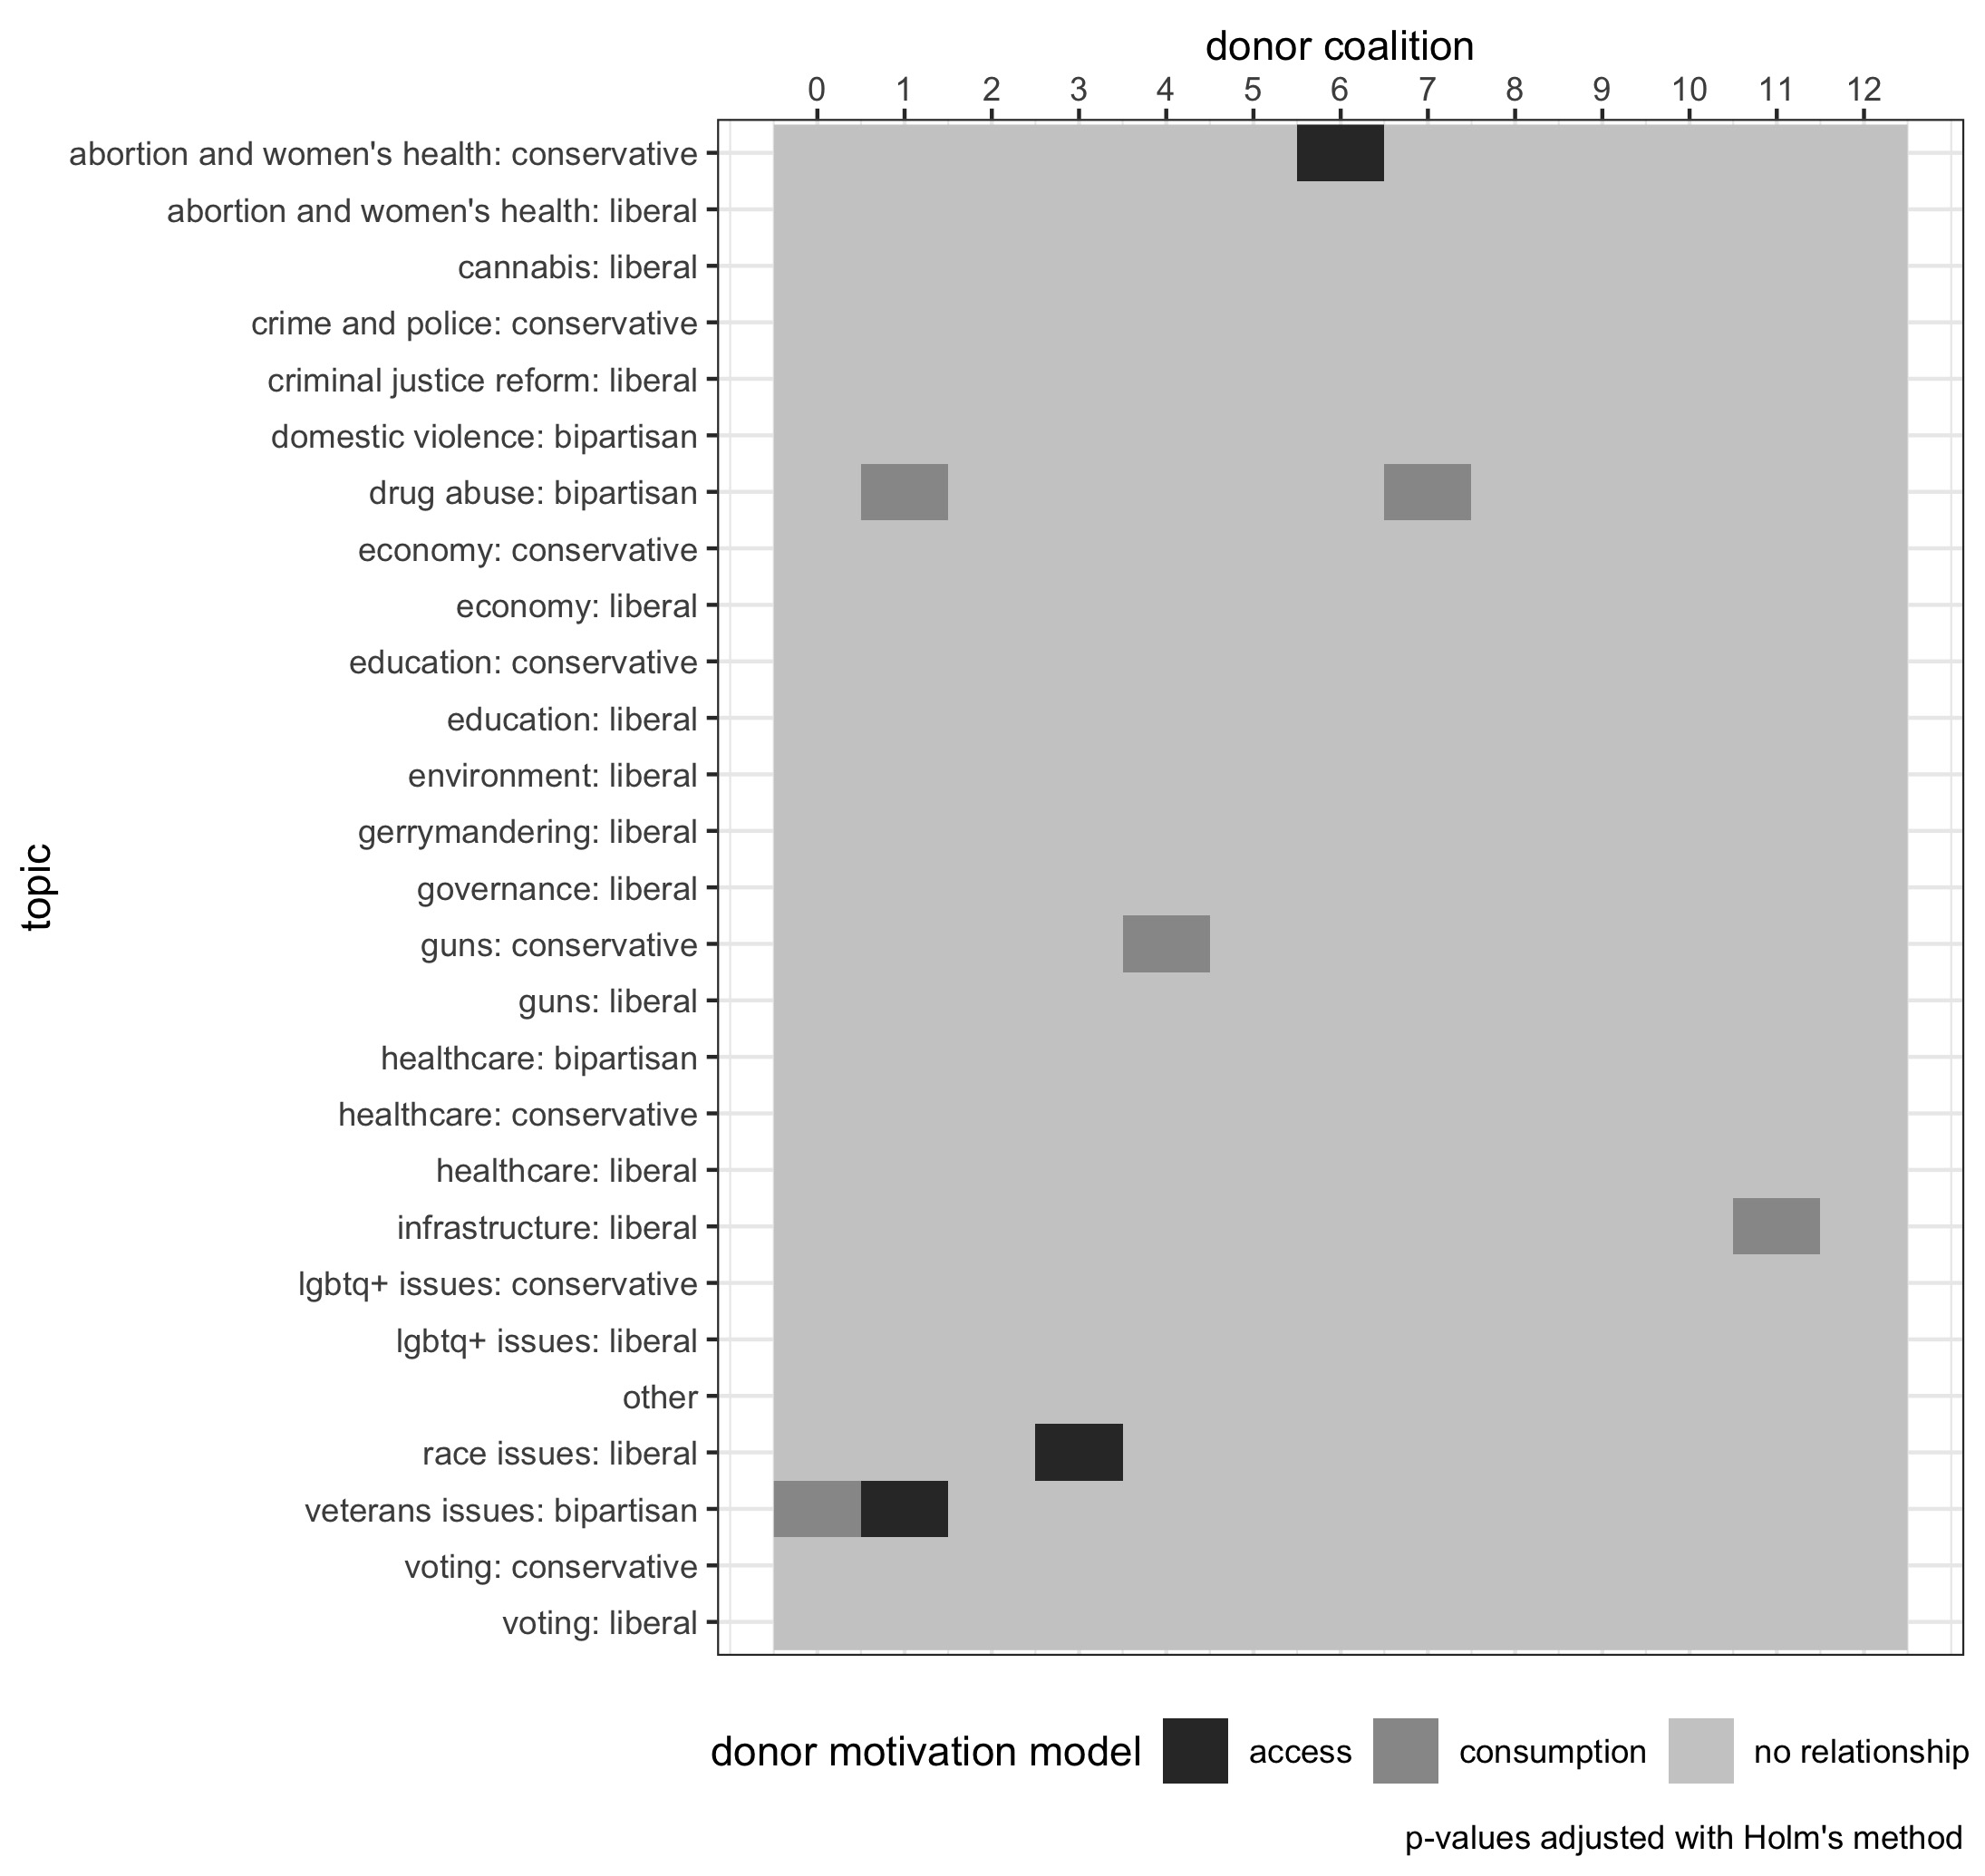
\includegraphics{../tables_and_figures/fig_2.jpg}
\caption{Donor Motivation Models}
\end{figure}

There are three donor coalitions that show behavior consistent with the
access-oriented model. For these three groups and policy issues,
\(H_{1a}\) is accepted. These access-oriented coalitions represent 1,572
individual donors or 21.3\% of all donors in the dataset; 6,489
individual donations or 22.4\% of donations; and \$654,577.60 or 16.5\%
of dollars contributed. Each of these three coalitions appear to have
unique policy and even ideological positions that they support.

In addition to these three access-oriented clusters of donors, five
coalitions of donors exhibit behavior that one would expect under the
consumption model of donor motivations and are accepted by \(H_{1b}\).
In other words, public support of various policy issues from campaigns
predicts donations from these coalitions. The five consumption-motivated
clusters of donors contain: 2,702 (36.7\%) of donors; 11,080 (38.4\%) of
donations; and donated a collective \$1,341,129.70 (33.8\%) of money
contributed. Similar to access-oriented clusters, consumption-oriented
coalitions show significant relationships to policy issues across the
ideological spectrum.

These results were used to test \(H_{1a}\) and \(H_{1b}\). Donor
coalitions and the topic of social media posts that were accepted by
\(H_{1a}\) and \(H_{1b}\) are listed in Table 1.

\hypertarget{donor-sizes}{%
\subsection{Donor Sizes}\label{donor-sizes}}

Coalitions of donors that were accepted by only \(H_{1a}\) or \(H_{1b}\)
were used to test \(H_{2a}\), that access-oriented donors are on-average
larger donors, and \(H_{2b}\), that consumption-oriented donors are
on-average smaller donors, with a difference-in-means permutation test.
A non-parametric bootstrap was used since the statistical assumptions
were not met for an OLS regression. Results to \(H_{2a}\) and \(H_{2b}\)
are in Table 2. Neither the access-oriented donors nor the
consumption-oriented donors contributed statistically significantly
different amounts of money than the other donors.

\begin{longtable}[]{@{}llrlr@{}}
\caption{Difference in Average Donor Size}\tabularnewline
\toprule
Hypothesis & Model & Avg. Diff & 95\% CI & p-value \\
\midrule
\endfirsthead
\toprule
Hypothesis & Model & Avg. Diff & 95\% CI & p-value \\
\midrule
\endhead
\(H_{2a}\) & access & -48.62 & -115.4, 21.47 & 0.144 \\
\(H_{2b}\) & consumption & 34.60 & -29.21, 118.39 & 0.310 \\
\bottomrule
\end{longtable}

A histogram showing the total contributions of donors by motivational
model are in Figure 3.

\begin{figure}
\centering
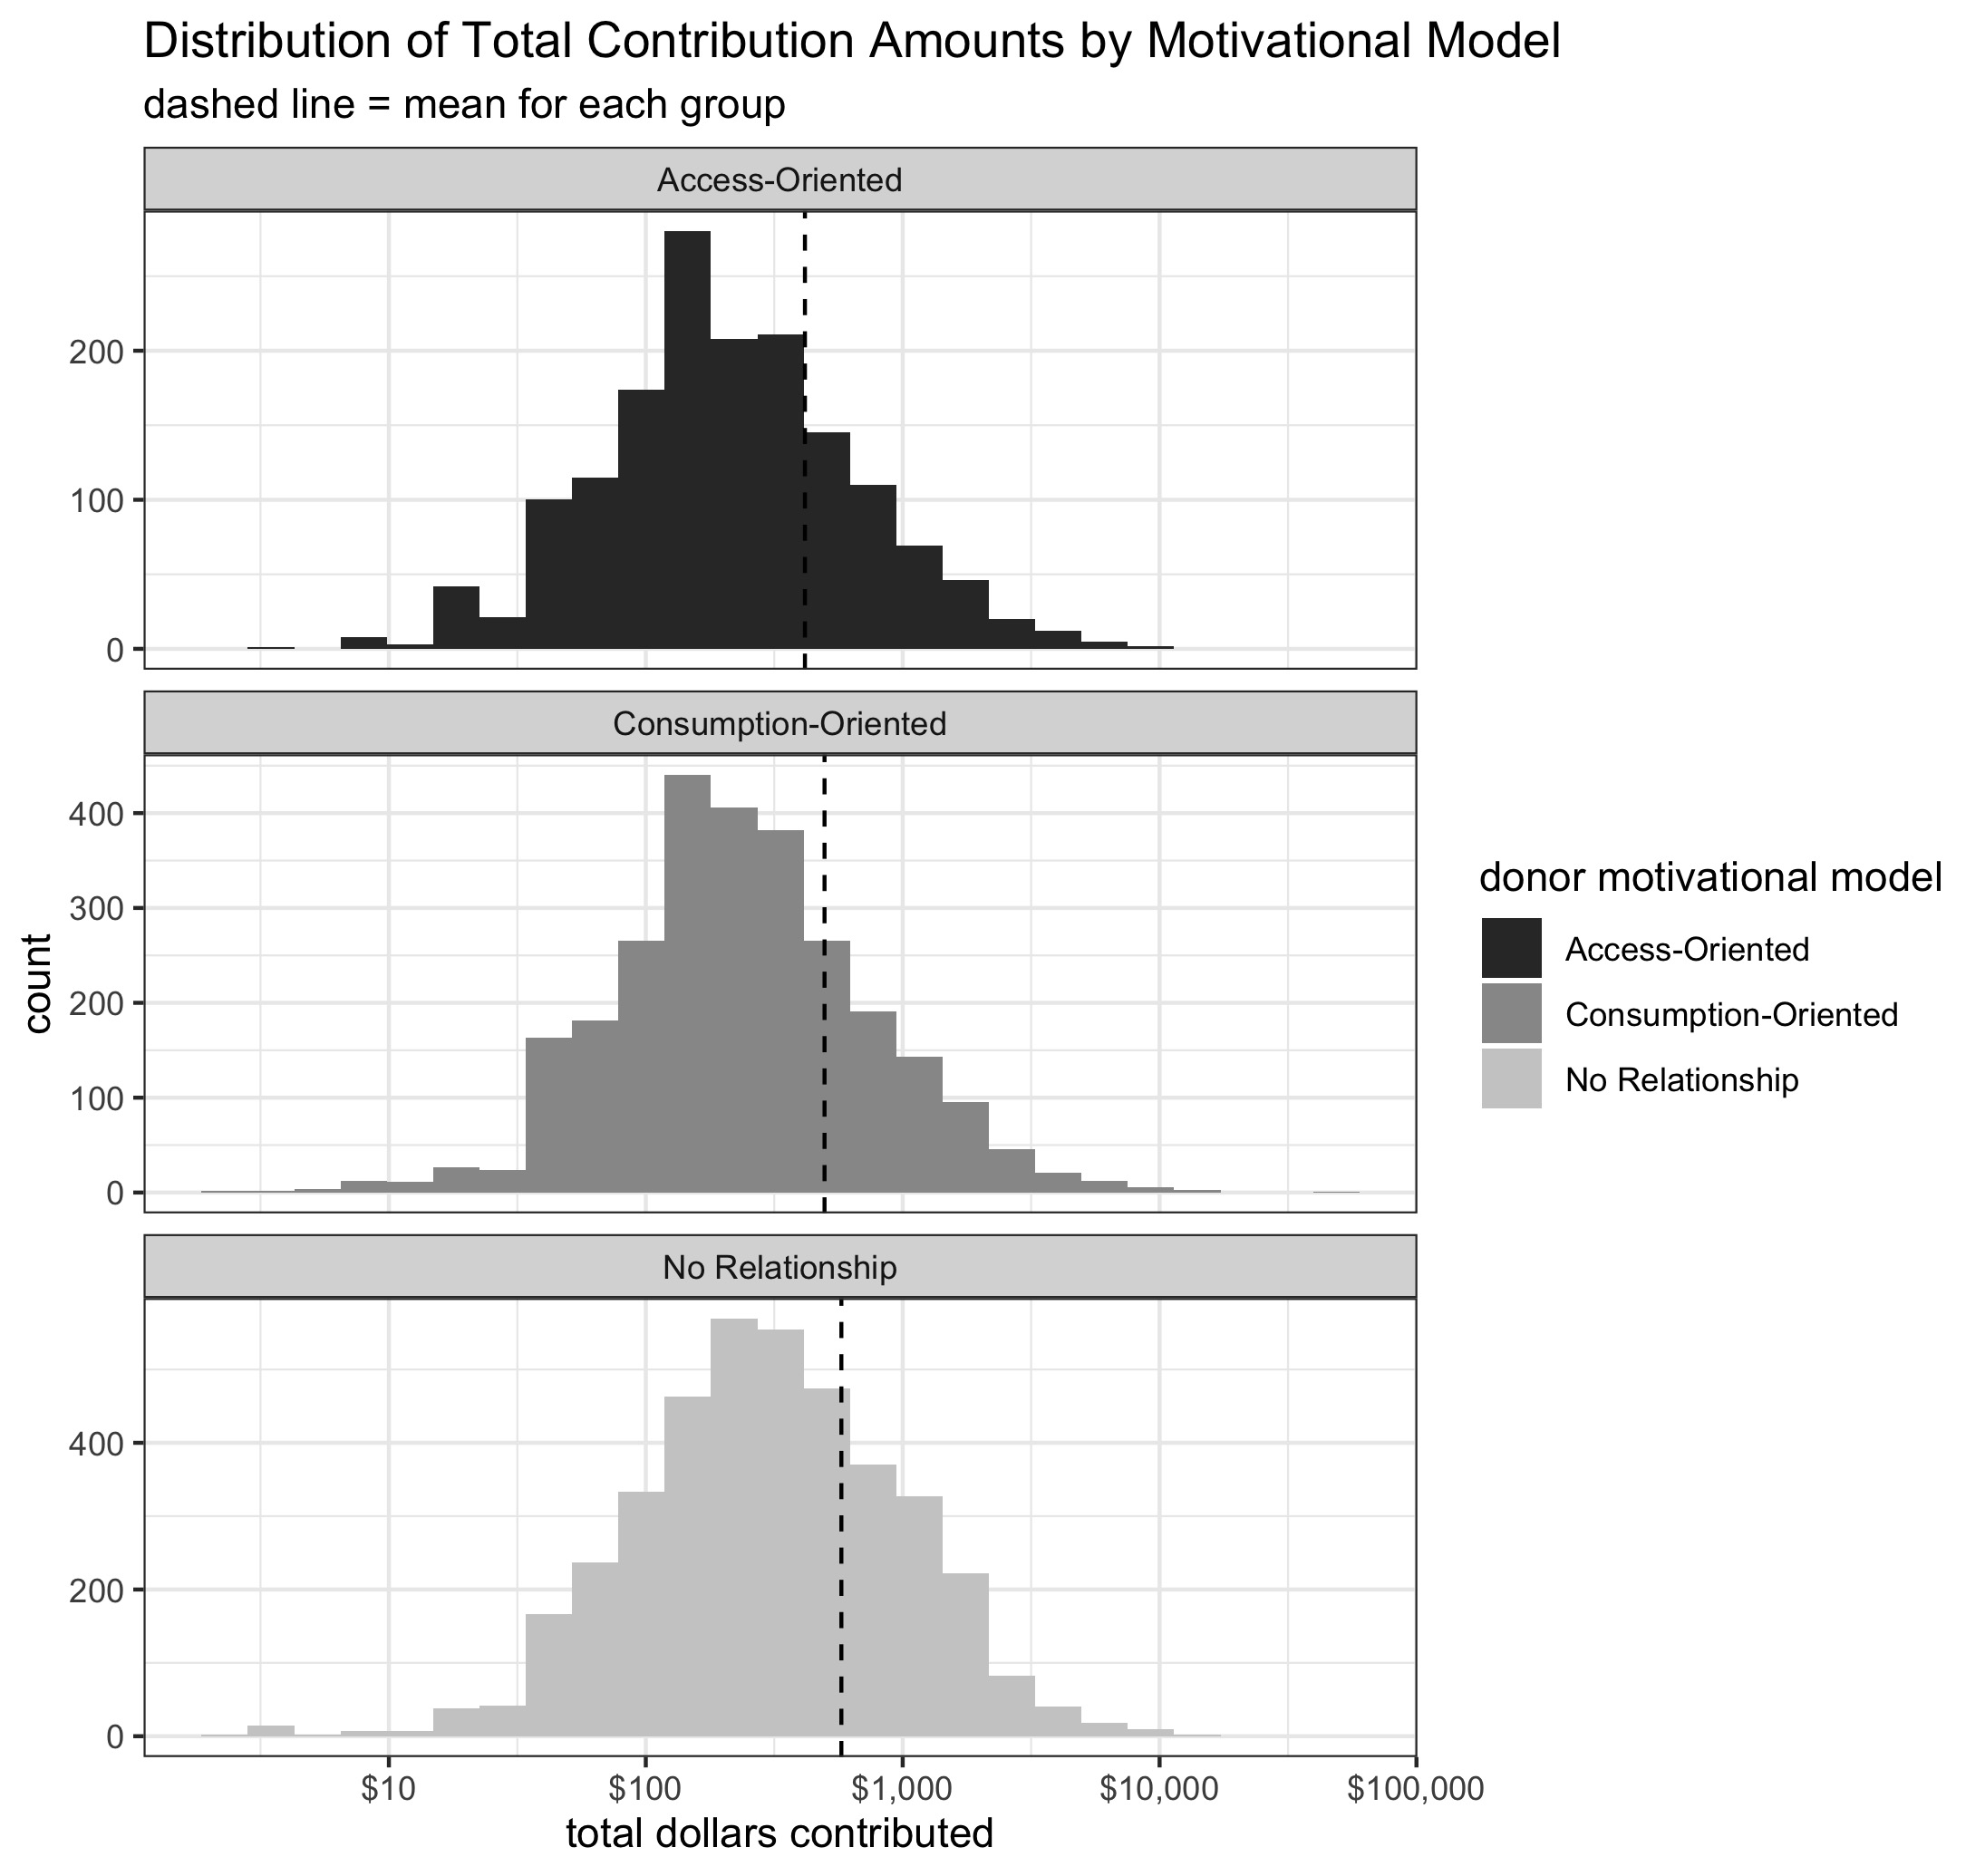
\includegraphics{../tables_and_figures/fig_donor_sizes.jpg}
\caption{Amount contributed by each donor in the dataset by motivational
model.}
\end{figure}

\hypertarget{donor-spatial-positions}{%
\subsection{Donor Spatial Positions}\label{donor-spatial-positions}}

To study the polarization of consumption-motivated donors, I extract the
x-coordinate, the axis of ideological position, from the donor network
(Figure 1). The positions of all the donors grouped by motivational
model is shown in Figure 4.

\begin{figure}
\centering
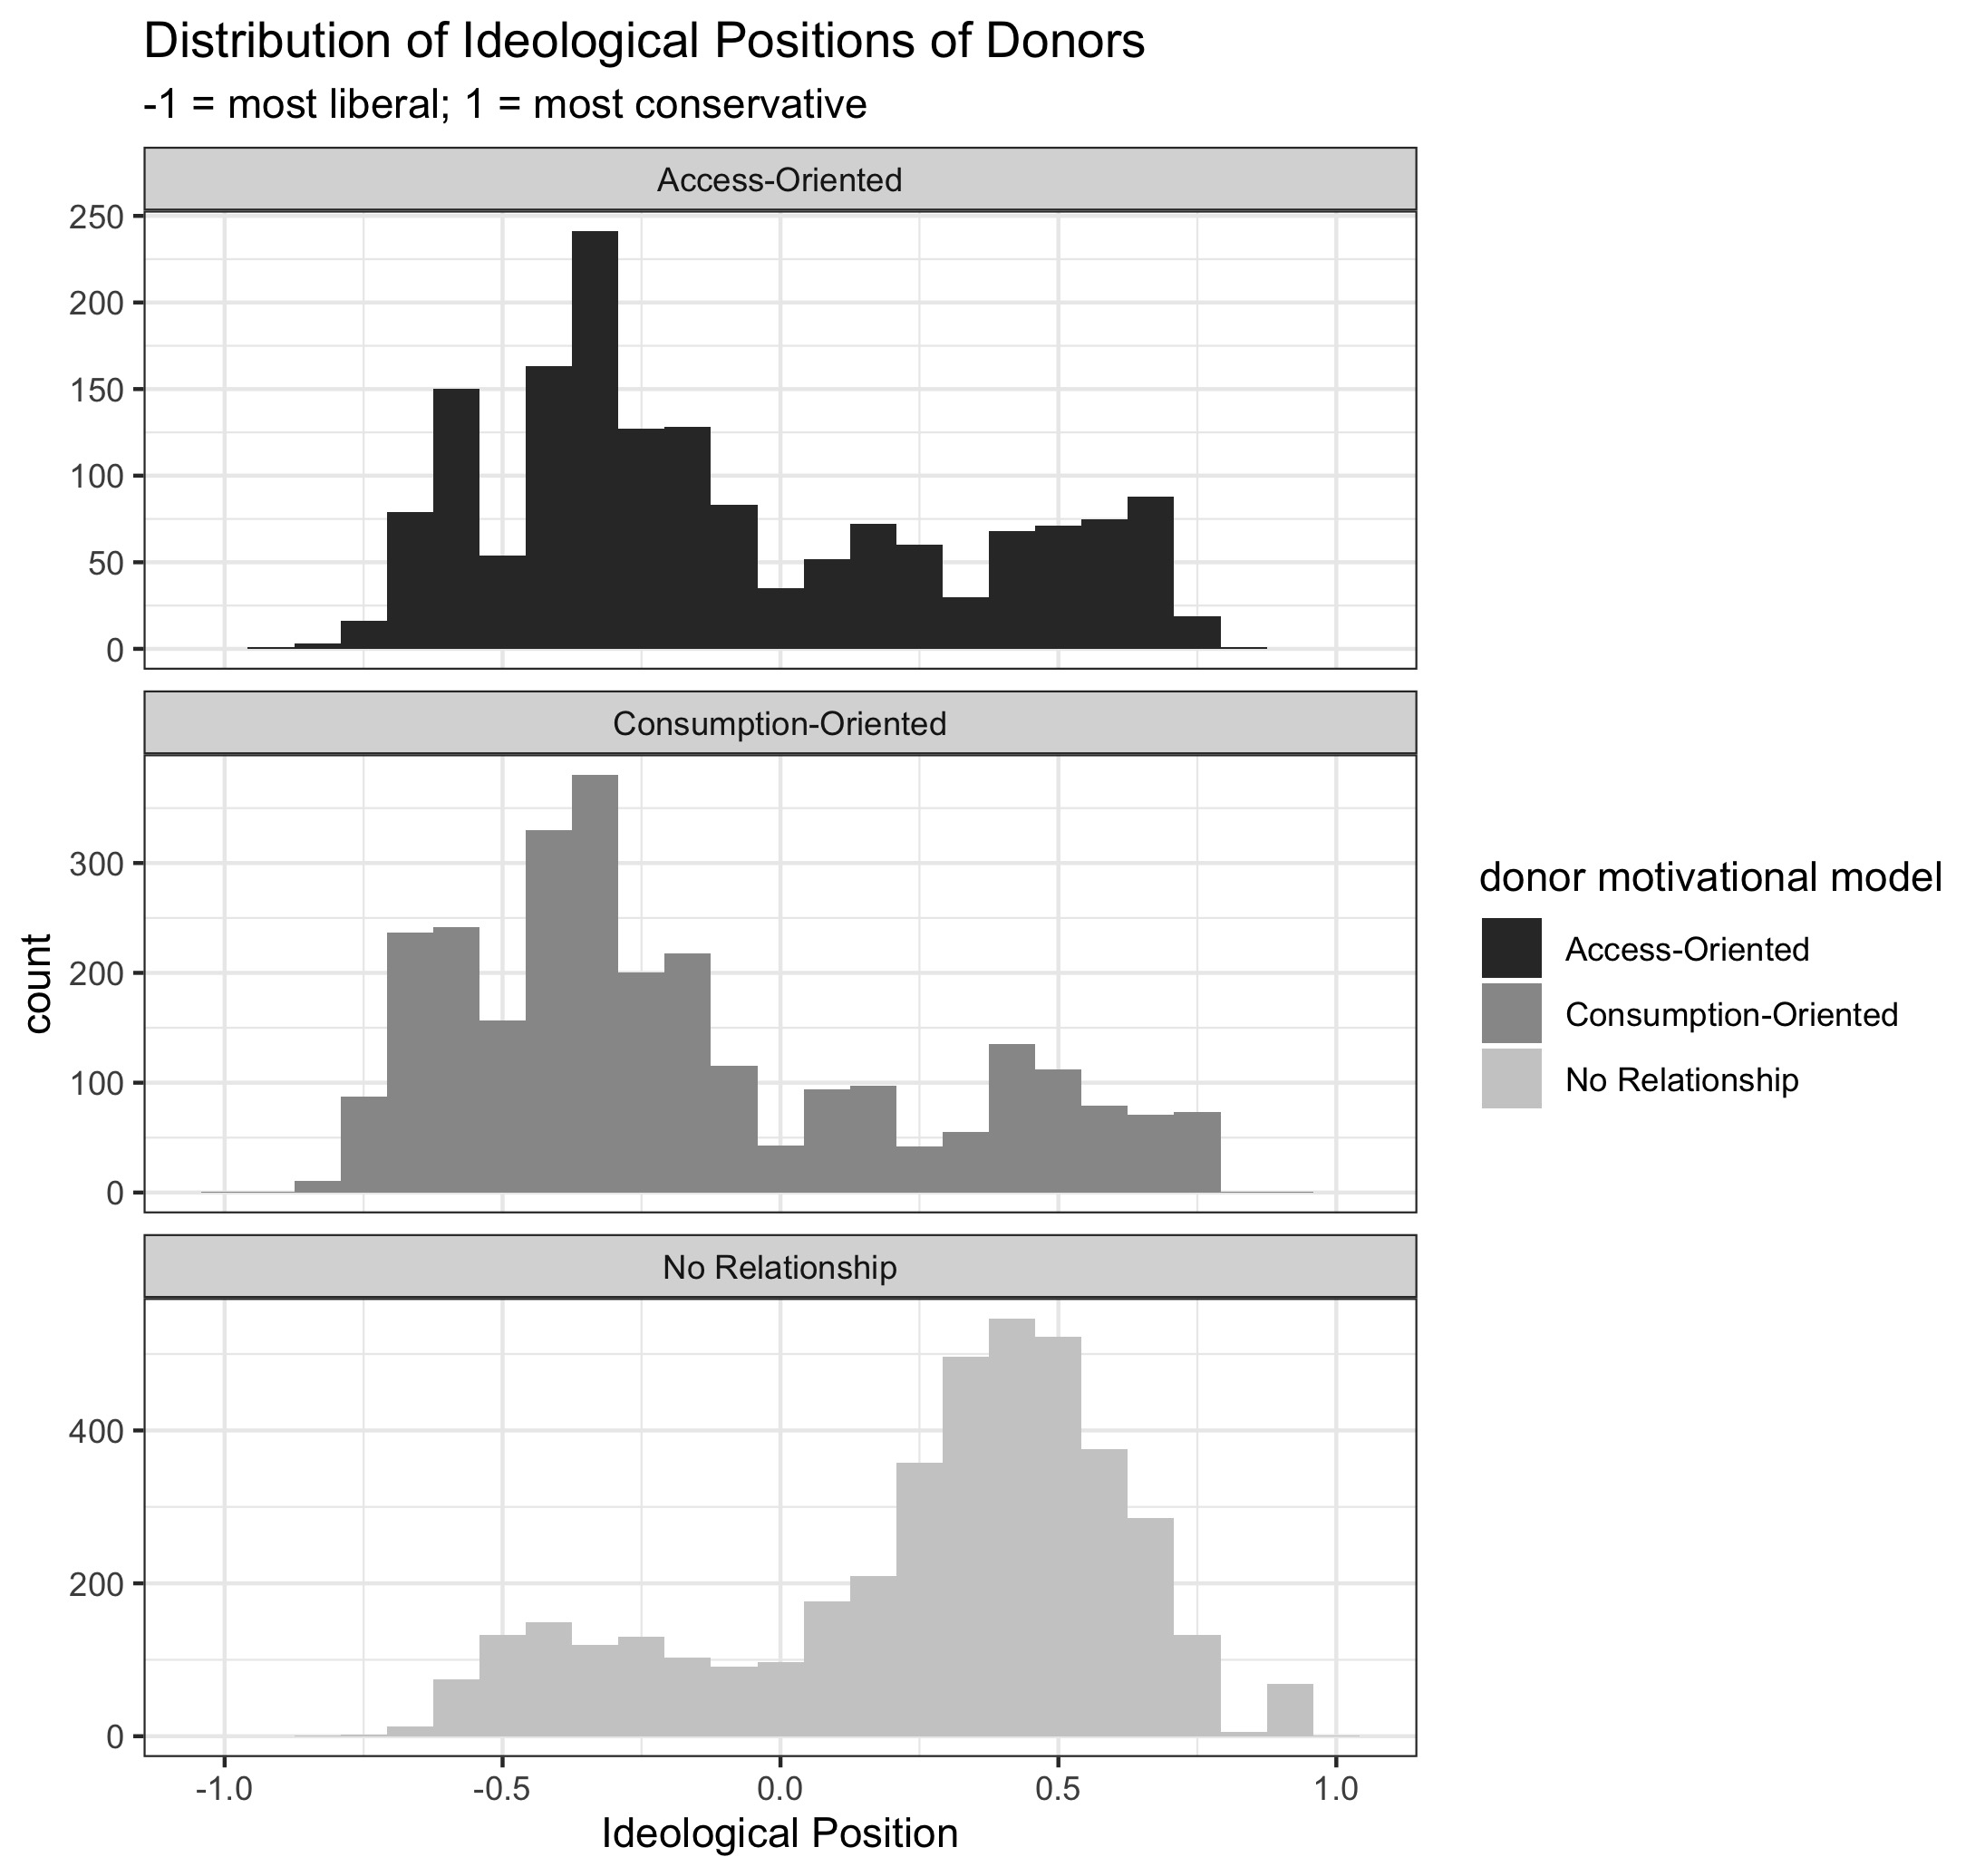
\includegraphics{../tables_and_figures/fig_node_position.jpg}
\caption{Spatial position along the ideological x-axis of each donor.}
\end{figure}

Table 3 shows the breakdown of donors who contribute a majority of their
money to Democrats and Republicans by motivational model.

\begin{longtable}[]{@{}lll@{}}
\caption{Percent of donors categorized as each motivational model who
contributed a majority of their money to Republicans and
Democrats}\tabularnewline
\toprule
Motivational Model & \% Republican & \% Democrat \\
\midrule
\endfirsthead
\toprule
Motivational Model & \% Republican & \% Democrat \\
\midrule
\endhead
Access-Oriented only & 63.9\% & 36.1\% \\
Consumption-Oriented only & 34.7\% & 65.3\% \\
No Relationship & 74.7\% & 25.3\% \\
\bottomrule
\end{longtable}

I then rescale the coordinate position to be -1 to 1, with -1
representing the most Democratic node and 1 representing the most
Republican node. To test \(H_{3a}\), that consumption-oriented donors
are more polarized in the network graph, and \(H_{3b}\), that
access-oriented donors are less polarized in the network graph, a
difference-in-means permutation test was conducted on the absolute value
of the rescaled x-coordinate with the coalition category as a variable.
A non-parametric permutation test was used since the statistical
assumptions for an OLS regression were not met. This absolute value
effectively is the level of polarization in the graph, with the nodes
that are on the extremes of the graph being closer to 1 and the
central-most nodes, representing bipartisan donors, being closer to 0.
Results for \(H_{3a}\) and \(H_{3b}\) are in Table 4.
Consumption-motivated donors are on average in more polarized positions
(further to the left and right of the graph) than
non-consumption-oriented donors, and access-oriented donors are on
average in less polarized positions (closer to the middle of the graph)
than non-access-oriented donors.

\begin{longtable}[]{@{}llrll@{}}
\caption{Difference in Average Donor Position
Polarization}\tabularnewline
\toprule
Hypothesis & Model & Avg. Diff & 95\% CI & p-value \\
\midrule
\endfirsthead
\toprule
Hypothesis & Model & Avg. Diff & 95\% CI & p-value \\
\midrule
\endhead
\(H_{3a}\) & access & -0.05 & -0.06, -0.03 & \textless.001 \\
\(H_{3b}\) & consumption & 0.01 & 0, 0.02 & 0.014 \\
\bottomrule
\end{longtable}

The polarized positions of all the donors are shown by group in Figure
5.

\begin{figure}
\centering
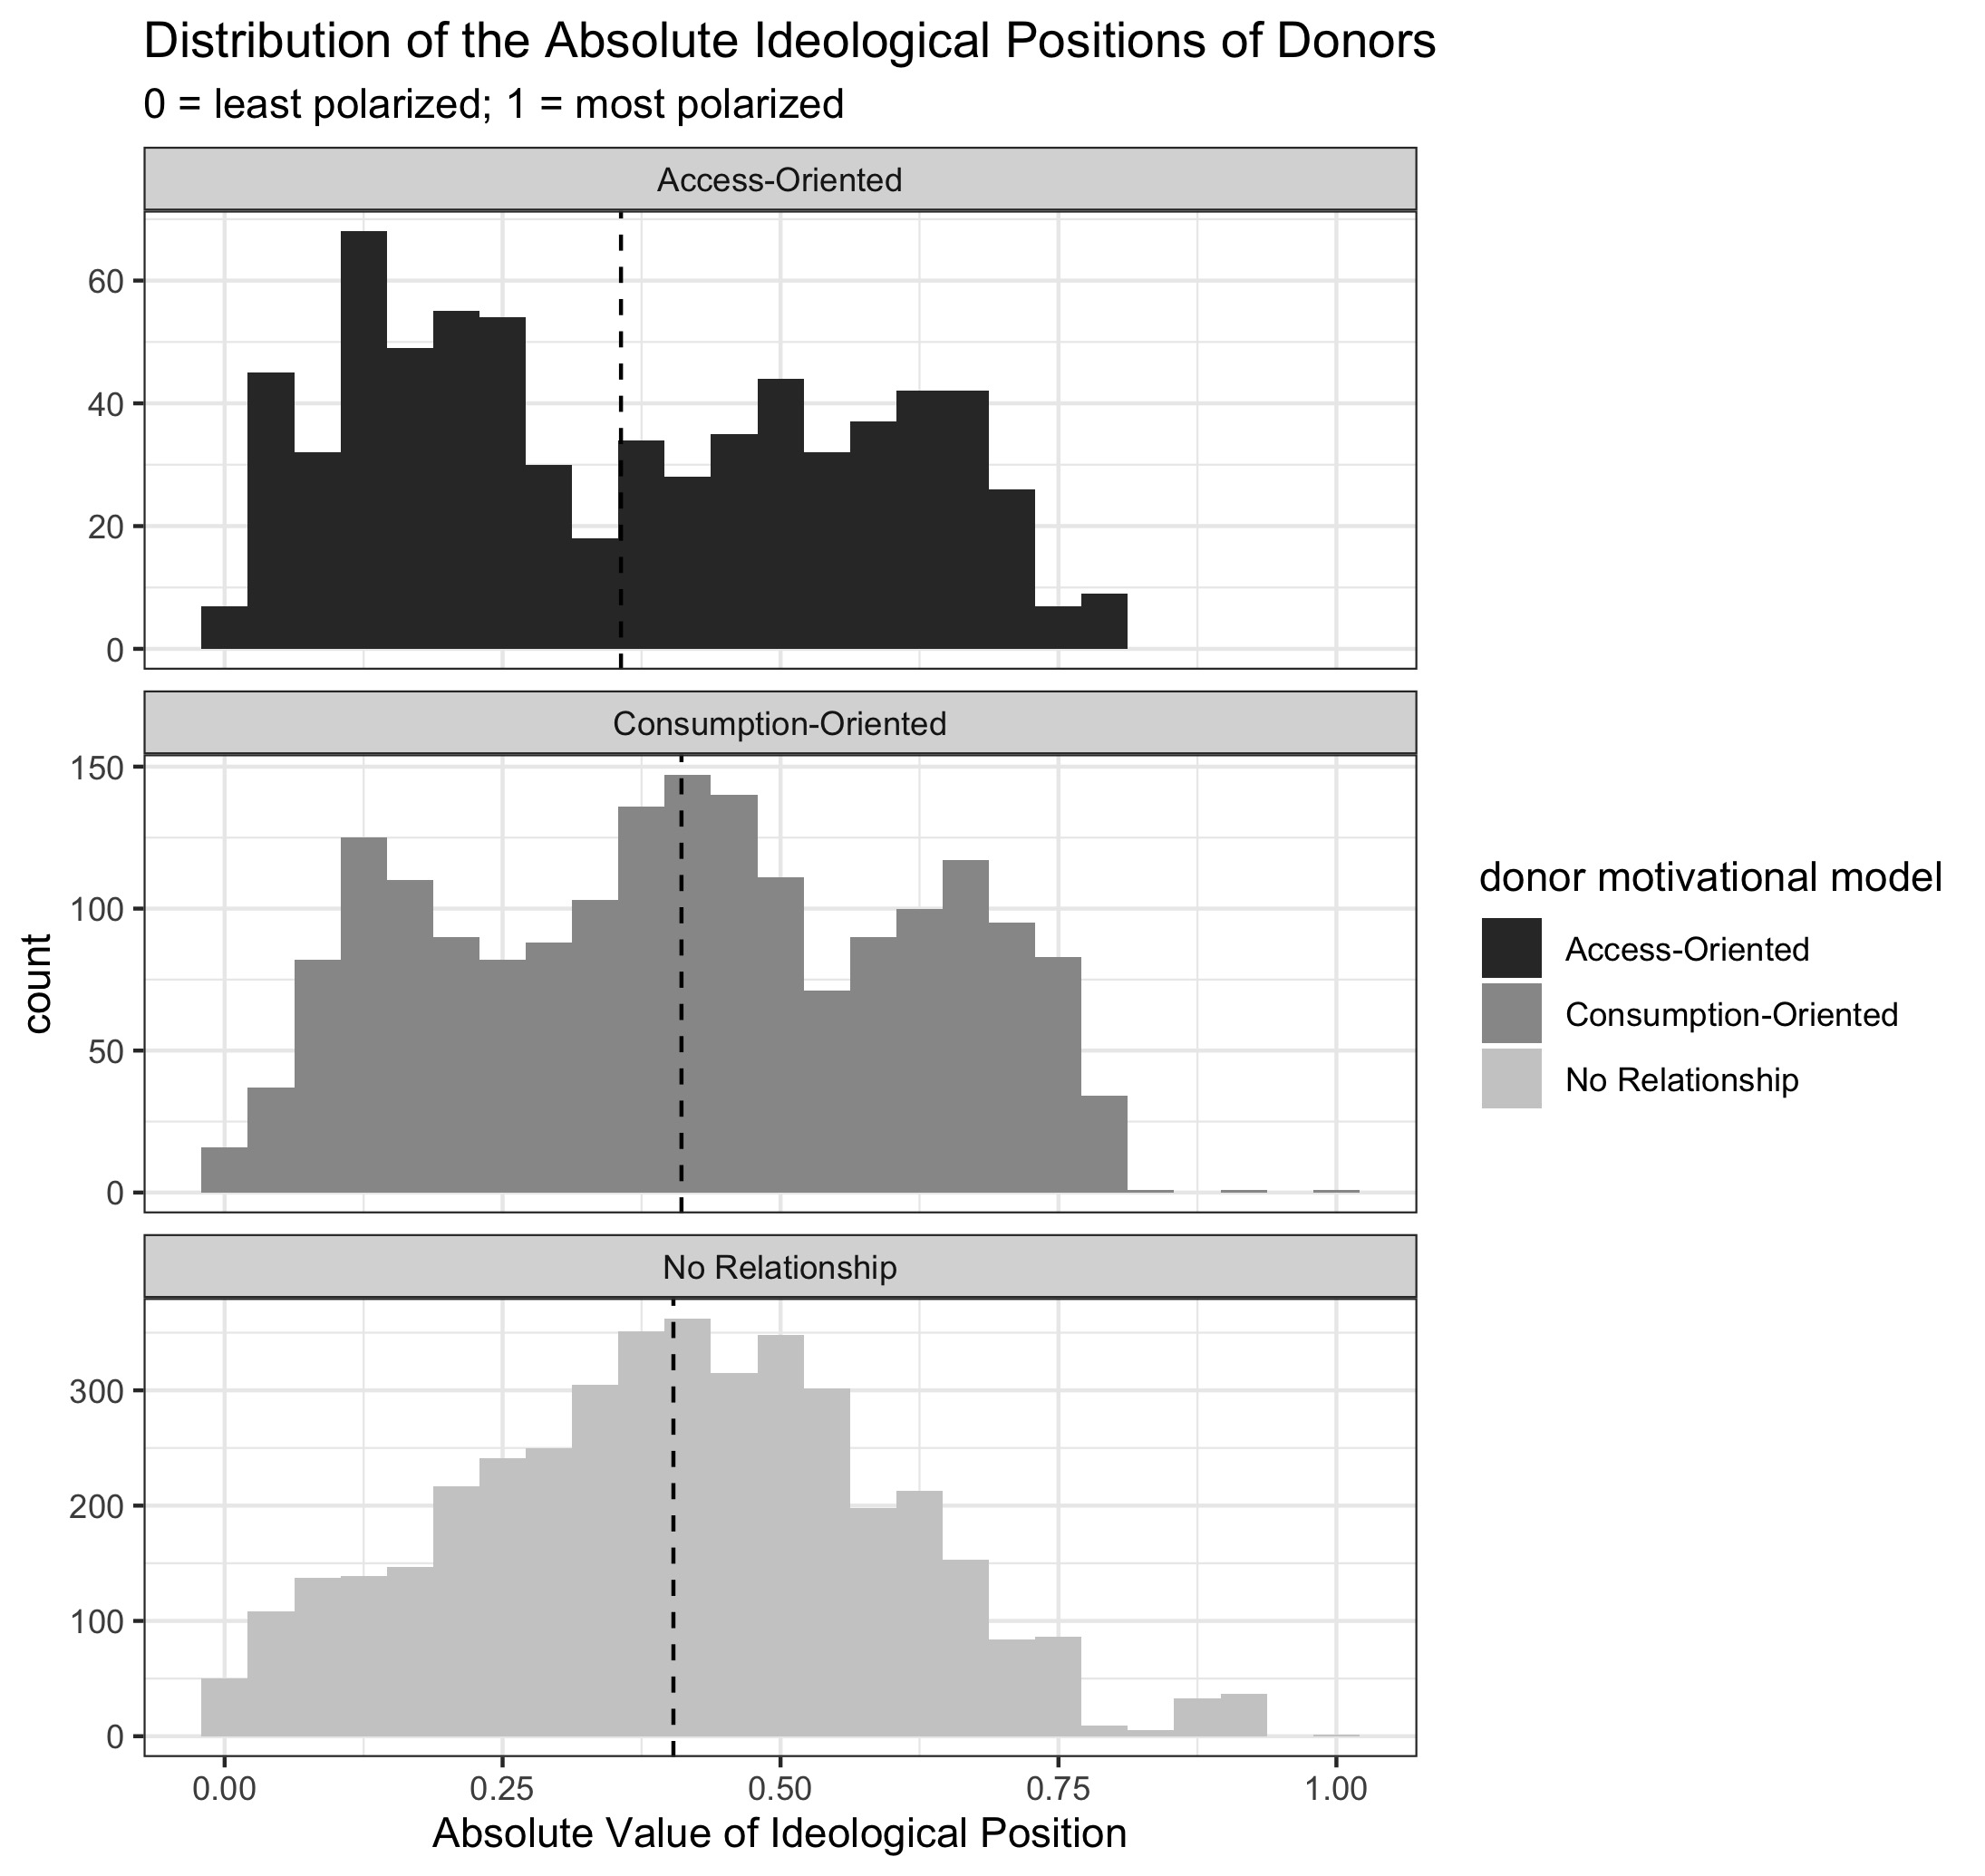
\includegraphics{../tables_and_figures/fig_node_position_absolute.jpg}
\caption{Polarized spatial position of each donor.}
\end{figure}

\hypertarget{discussion}{%
\section{Discussion}\label{discussion}}

I find evidence that eschews historical scholarship that political
donors are monolithic in their motivations. Instead, I find that
different donors hold different motivations.

Different donor coalitions exhibited behavior that is in line with both
the access-oriented and consumption model of political donations with
policy issues across the ideological spectrum of liberal, conservative,
and bipartisan. Example social media posts of the various topics can be
found in the appendix.

While much of the popular concern over money in politics is around
access-oriented donors manipulating the political system, I find that
there are more consumption-oriented--rather than access-oriented--donors
(2,702 versus 1,572), donations (11,080 versus 6,489), and total amount
contributed by each type (\$1,341,129.70 versus \$654,577.60). While any
number of access-oriented donors may remain concerning to some in the
public, these results suggest that more people use political donations
as a vehicle for increased participation in, not manipulation of, the
political process.

One idea about political donors is that access-oriented donors are
large-dollar donors with financial incentives, but the results of
\(H_{2a}\) reject this idea in the context of the 2016 elections in
Wisconsin. Donors in access-oriented coalitions do not contribute
statistically significantly more money on-average than other donors.
Just because a donor is not contributing a large sum of money themselves
does not mean that they are not seeking to coax a politician into
supporting specific policies. This attempt at influence can be amplified
when coalitions of donors operate in conjunction with one another. For
example, members of an interest group could each contribute a relatively
small amount of money, but in the aggregate, the unified donations could
potentially gain that interest group access to a politician. A future
study could replicate this analysis with multiple election cycles or
study multiple states or federal elections to achieve higher statistical
power.

The stereotype of consumption-motivated donors is of small-dollar donors
whose contributions are harnessed online. Similar to access-oriented
donors, \(H_{2b}\) is rejected and consumption-motivated donors are not
on-average smaller donors than other contributors. Again, these results
suggest a rethinking of the notion that the amount of money one
contributes is indicative of one's motivations. If someone is able to
contribute a large sum of money and they care about a certain issue, it
stands to reason that they may just support politicians who already care
about that issue. This paper challenges conventional beliefs on the size
of access-oriented versus consumptive donors.

In contrast, this paper concurs with the literature that
consumption-motivated donors are in more polarized spatial positions
within the donor graph than non-consumptive donors. Access-oriented
donors are more centrally located. The acceptances of \(H_{3a}\) and
\(H_{3b}\) are in agreement with past literature. These results provide
descriptive context and are not meant to imply any level of causality.
Past studies have either suggested or found a connection between donor
motivations and political polarization, and this study also finds these
descriptive relationships. Future studies should examine the causal
mechanisms of these relationships. Do candidates take more polarizing
stances in an effort to court consumptive donors? Has an increased
number of consumptive donors helped more polarized candidates to win
office? Do access-oriented donors seek out campaigns that are more
moderate? Or can access-oriented donors influence the ideological
extremity of candidates?

In addition to the finding that both models can exist in different donor
coalitions, it is also possible that the same cluster can operate under
both models. One of the thirteen donor clusters, coalition 1, revealed a
duality where they were access-oriented in relation to one policy issue
and consumption-oriented in relation to another. While it is possible
that this finding is statistical noise, there is additional face
validity because the two issues the donor coalition had a relationship
with were both bipartisan issues--veterans issues and drug abuse. Few
studies have come to the conclusion that donors can operate with both
motivational models. While this study finds this behavior to be
relatively rare, in only one donor cluster, it hints to a more complex
view as to why donors make a political contribution. Further, public
support of one policy issue, veteran's issues, is both Granger caused by
donations from a coalition and Granger causes another coalition to make
a contribution. This result suggests that issues can play different
roles to different groups of political donors. One group of donors can
seek access to influence a policy, and another group can display
consumptive behavior and reward politicians who already publicly support
that policy.

Finally, there has been a debate among campaign-finance scholars as to
whether donation motivations are driven by only ideological proximity or
specific policy issues. I find that policy issues are a factor in
contribution motivations, at least for the specific groups that exhibit
access-oriented or consumptive behavior. The policy issues that are
connected to donor clusters in this study range the political spectrum,
including liberal policies (race issues, public infrastructure),
conservative policies (pro-life, pro-gun), and bipartisan issues (drug
abuse, veteran's issues). Further, some of the topics are perennial
focuses of campaigns, such as pro-life politics. Other issues were
particularly salient during this election cycle, such as veterans issues
with the Tomah Veterans' Affair hospital scandal (Honl 2016) and King
Veterans' Home scandal. These two scandals created an electoral
environment in which veterans' issues were in the public focus, and
results from this paper suggest that some political donors both sought
to influence campaigns to address these issues as well as reward
politicians for their focus on the topic.

Six of the thirteen coalitions of donors did not display access-oriented
or consumption-oriented behavior with the policy topics tested. The
motivations behind these clusters of donors remain unclear. It is
possible that they are motivated by ideological proximity in a way that
is not adequately tested using the methods in this paper. Future studies
should test other potential reasons that people make political
contributions, such as individuals contributing to ideologically
proximate campaigns, geographically local campaigns, competitive
campaigns, or other potential motivations.

\hypertarget{limitations}{%
\section{Limitations}\label{limitations}}

Like all observational studies, this research cannot claim true
causality. While the main methodology employed is formally called
``Granger causality,'' this causality is in an econometric sense and is
more akin to predictive value. So while the findings of this paper do
have predictive power--for example, donations from certain groups of
individuals successfully receiving candidates to publicly support policy
issues--true causal claims cannot be made. Future studies should use the
findings from this research to conduct lab experiments where causal
claims can be made.

I found discrete examples of donor coalitions demonstrating
access-oriented or consumptive behavior on specific issues. However,
these results do not suggest that these donors only care about those
issues or that other donors do not care about these issues. Instead,
these donors have a unique statistical relationship where when they
contribute money to a political campaign, it either predicts or is
predicted by campaigns' public support of policy issues. Future studies
can employ surveys to identify if the statistical relationships found in
an analysis like this present work concur with people's self
conceptions. Do donor coalitions who donate in a consumptive fashion,
that is where they contribute to a campaign after they publicly support
an issue, actually report that they prioritize that issue? Possibly,
these behaviors are subconscious reactions. Donors may not be able to
exactly identify \emph{why} they like a candidate or may report some
other reason, when it is actually a reinforcement of a concurrence
between their policies and the information environment that they
consume.

Finally, this study was not meant to find nor did it find exhaustive
evidence as to what motivates ever single donor in the dataset. Even
within the information ecology, this study does not consider things like
news stories or personal friend circles. Moreover, there are other
potential reasons that donors make contributions, such as geographic
proximity where people donate to their local candidates or allocating
money to competitive races. Future research can consider these other
variables as possible explanations for political donations.

\hypertarget{conclusion}{%
\section{Conclusion}\label{conclusion}}

Campaign finance scholars are divided on the motivations of political
donors. Do political donors seek to buy access, to participate more in
politics, or some combination of both? This study finds that different
coalitions of donors, and in one instance, a singular coalition, exhibit
behavior that is consistent with different motivational models. Overall,
there are more consumptive donors compared to access-oriented donors. In
addition, there is no statistical difference in the average contributor
size of access-oriented and consumption-oriented donors compared to
other donors. However, access-oriented donors are found to be more
spatially central within donor networks, and consumptive donors are more
polarized. While past research has largely treated political donors as a
monolith, with the possibility of operating under a single, I find that
different donors can have different motivational models.

\newpage

\hypertarget{appendix}{%
\section{Appendix}\label{appendix}}

\begin{longtable}[t]{>{\raggedright\arraybackslash}p{.65in}|>{\raggedright\arraybackslash}p{1in}|>{\raggedright\arraybackslash}p{1in}|>{\raggedright\arraybackslash}p{.7in}|>{\raggedright\arraybackslash}p{2.5in}}
\caption{\label{tab:unnamed-chunk-6}Social Media Examples}\\
\hline
example \# & topic & campaign & social media site & post\\
\hline
\endfirsthead
\caption[]{Social Media Examples \textit{(continued)}}\\
\hline
example \# & topic & campaign & social media site & post\\
\hline
\endhead
1 & race issues: liberal & Bowen 4 Action & Twitter & @ JoyAnnReid: \#OscarsSoWhite black people can't even get nominated for the movies about black people...\\
\hline
2 & race issues: liberal & Citizens of the 81st for Dave Considine & Twitter & 1 in every 9 African-Americans are disenfranchised because of felony convictions in Wisconsin\\
\hline
3 & abortion and women's issues: conservative & Ken Skowronski for Assembly & Facebook & Last night I had a great time at the Wisconsin Right to Life Dinner with my fellow colleagues. I am proud to have supported the bold Pro-Life reforms we have put in place and I will continue to defend the rights of those who cannot defend themselves.\\
\hline
4 & abortion and women's issues: conservative & Friends \& Neighbors of Robin Vos & Twitter & An Assembly committee will vote on a bill to ban the sale of aborted children's body parts on Wednesday.\\
\hline
5 & abortion and women's issues: conservative & Friends of Chuck Wichgers & Facebook & 'I'm glad to know Chuck, who is a solid conservative. He's shown that he understands the principles that secure our freedom and that he will work for them in office. But more than that, I've seen that he is passionate about the God-given dignity of every human life. He knows that every person's right to live and to live freely comes from a much higher source than government.'PATRICK MCILHERAN, FORMER EDITORIAL WRITER, MILWAUKEE JOURNAL SENTINEL\\
\hline
6 & veterans issues: bipartisan & Sanfelippo for Assembly & Twitter & Welcome Home Veterans Initiative seeks to solve veteran homelessness in state:\\
\hline
7 & veterans issues: bipartisan & Citizens for Peter Barca & Twitter & Regionalizing Wisconsin's county veterans service offices remains a concern in vet community\\
\hline
8 & guns: conservative & Scott Fitzgerald for Senate & Twitter & Thanks to the Wisconsin Game Preserve Association for the honor of their 2015 Legislator of the Year award!\\
\hline
9 & guns: conservative & Kremer for Wisconsin & Facebook & This is a fair interview with Frederica Freyberg discussing the 'Campus Carry Act' in Wisconsin.  This aired on public television yesterday morning.\\
\hline
10 & infrastructure: liberal & Friends of Jonathan Brostoff & Facebook & Dr. Mark Stout has written a compelling alternative to the \$1.1 billion highway proposal. This option that would save money and provide a brighter, more progressive, more responsible future for our state. If you haven't yet, please take a look and share widely.\\
\hline
11 & infrastructure: liberal & Wachs for Assembly & Twitter & WI roads rank 3rd worst in US. Yet Scott Walker isnt ready to put politics aside to solve our infrastructure woes.\\
\hline
12 & drug abuse: bipartisan & Michael Schraa for Assembly & Facebook & A great story about the HOPE Agenda and my colleague on Joint Finance, WI State Rep John Nygren's efforts to fight against heroin and opiate addiction.\\
\hline
\end{longtable}

\begin{tabular}{l|l|l}
\hline
Method & koRpus & stringi\\
\hline
Word count & 5272 & 5248\\
\hline
Character count & 35323 & 35337\\
\hline
Sentence count & 276 & Not available\\
\hline
Reading time & 26.4 minutes & 26.2 minutes\\
\hline
\end{tabular}

\newpage

\hypertarget{references}{%
\section*{References}\label{references}}
\addcontentsline{toc}{section}{References}

\hypertarget{refs}{}
\begin{CSLReferences}{1}{0}
\leavevmode\vadjust pre{\hypertarget{ref-bic}{}}%
Ahelegbey, Daniel Felix, Monica Billio, and Roberto Casarin. 2016.
{``Bayesian graphical models for STructural vector autoregressive
processes.''} \emph{Journal of Applied Econometrics} 31(2): 357--386.
doi: \href{https://doi.org/10.1002/jae.2443}{10.1002/jae.2443}.

\leavevmode\vadjust pre{\hypertarget{ref-akey2015}{}}%
Akey, Pat. 2015. {``{Valuing Changes in Political Networks: Evidence
from Campaign Contributions to Close Congressional Elections}.''}
\emph{The Review of Financial Studies} 28(11): 3188--3223. doi:
\href{https://doi.org/10.1093/rfs/hhv035}{10.1093/rfs/hhv035}.

\leavevmode\vadjust pre{\hypertarget{ref-albert2020}{}}%
Albert, Zachary, and Raymond La Raja. 2020. {``Small dollar donors and
the evolving democratic party.''} \emph{APSA Preprints}. doi:
\href{https://doi.org/10.33774/apsa-2020-9rnkd}{10.33774/apsa-2020-9rnkd}.

\leavevmode\vadjust pre{\hypertarget{ref-ansolabehere2003}{}}%
Ansolabehere, Stephen, John M. de Figueiredo, and James M. Snyder. 2003.
{``Why is there so little money in u.s. politics.''} \emph{Journal of
Economic Perspectives} 17(1): 105--130. www.jstor.org/stable/3216842.

\leavevmode\vadjust pre{\hypertarget{ref-arbour2020}{}}%
Arbour, Brian. 2020. {``Tiny donations, big impact: How small-dollar
donors are eroding the power of party insiders.''} \emph{Society} 57:
496--506. doi:
\href{https://doi.org/0.1007/s12115-020-00520-4}{0.1007/s12115-020-00520-4}.

\leavevmode\vadjust pre{\hypertarget{ref-arceneaux2009}{}}%
Arceneaux, Kevin, and David W. Nickerson. 2009. {``Who is mobilized to
vote? A re-analysis of 11 field experiments.''} \emph{American Journal
of Political Science} 53(1): 1--16. doi:
\href{https://doi.org/10.2307/25193864}{10.2307/25193864}.

\leavevmode\vadjust pre{\hypertarget{ref-baker2020a}{}}%
Baker, Anne. 2020. {``Policies, profits, networks, or duty?: Donors'
motivations for contributing to parties and interest groups.''}
\emph{The Social Science Journal} 0(0): 1--16. doi:
\href{https://doi.org/10.1080/03623319.2020.1727224}{10.1080/03623319.2020.1727224}.

\leavevmode\vadjust pre{\hypertarget{ref-barber2016a}{}}%
Barber, Michael. 2016. {``Donation motivations: Testing theories of
access and ideology.''} \emph{Political Research Quarterly} 69(1):
148--159. 10.1177/1065912915624164.

\leavevmode\vadjust pre{\hypertarget{ref-barber2017}{}}%
Barber, Michael J., Brandice Canes-Wrone, and Sharece Thrower. 2017.
{``Ideologically sophisticated donors: Which candidates do individual
contributors finance?''} \emph{American Journal of Political Science}
61(2): 271--288. doi:
\href{https://doi.org/10.1111/ajps.12275}{10.1111/ajps.12275}.

\leavevmode\vadjust pre{\hypertarget{ref-barber2019}{}}%
Barber, Michael, Brandice Canes-Wrone, and Sharece Thrower. 2019.
{``Campaign contributions and donors' policy agreement with presidential
candidates.''} \emph{Presidential Studies Quarterly} 49(4): 770--797.
doi: \href{https://doi.org/10.1111/psq.12609}{10.1111/psq.12609}.

\leavevmode\vadjust pre{\hypertarget{ref-rfacebook}{}}%
Barbera, Pablo, Andrew Geisler, and Wouter van Atteveldt. 2017.
\emph{Rfacebook}.
\url{https://cran.r-project.org/web/packages/Rfacebook/Rfacebook.pdf}.

\leavevmode\vadjust pre{\hypertarget{ref-gephi}{}}%
Bastian, Mathieu, Sebastien Heymann, and Mathieu Jacomy. 2009. {``Gephi:
An open source software for exploring and manipulating networks.''}
\url{http://www.aaai.org/ocs/index.php/ICWSM/09/paper/view/154}.

\leavevmode\vadjust pre{\hypertarget{ref-bastos2015}{}}%
Bastos, Marco T., Dan Mercea, and Arthur Charpentier. 2015. {``{Tents,
Tweets, and Events: The Interplay Between Ongoing Protests and Social
Media}.''} \emph{Journal of Communication} 65(2): 320--350. doi:
\href{https://doi.org/10.1111/jcom.12145}{10.1111/jcom.12145}.

\leavevmode\vadjust pre{\hypertarget{ref-bonica2016}{}}%
Bonica, Adam. 2016. {``Avenues of influence: On the political
expenditures of corporations and their directors and executives.''}
\emph{Business and Politics} 18(4): 367--394. doi:
\href{https://doi.org/10.1515/bap-2016-0004}{10.1515/bap-2016-0004}.

\leavevmode\vadjust pre{\hypertarget{ref-caneswrone2019}{}}%
Canes-Wrone, Brandice, and Nathan Gibson. 2019. {``Developments in
congressional responsiveness to donor opinion.''} In \emph{Can america
govern itself?}, SSRC anxieties of democracy, eds. Frances E. Lee and
NolanEditors McCarty. Cambridge University Press, p. 69--92. doi:
\href{https://doi.org/10.1017/9781108667357.004}{10.1017/9781108667357.004}.

\leavevmode\vadjust pre{\hypertarget{ref-choma2020}{}}%
Choma, Russ, and Kara Voght. 2020. {``Small-dollar donors powered the
2020 race. Then the pandemic happened.''} \emph{Mother Jones}.
\url{https://www.motherjones.com/politics/2020/04/small-dollar-donors-powered-the-2020-race-then-the-pandemic-happened/}.

\leavevmode\vadjust pre{\hypertarget{ref-constant2006}{}}%
Constant, Louay M. 2006. {``When money matters: Campaign contributions,
roll call votes, and school choice in florida.''} \emph{State Politics
\& Policy Quarterly} 6(2): 195--219. doi:
\href{https://doi.org/10.1177/153244000600600204}{10.1177/153244000600600204}.

\leavevmode\vadjust pre{\hypertarget{ref-cooper2010}{}}%
Cooper, Michael J., Huseyin Gulen, and Alexei V. Ovtchinnikov. 2010x.
{``Corporate political contributions and stock returns.''} \emph{The
Journal of Finance} 65(2): 687--724. doi:
\href{https://doi.org/10.1111/j.1540-6261.2009.01548.x}{10.1111/j.1540-6261.2009.01548.x}.

\leavevmode\vadjust pre{\hypertarget{ref-cranshaw2010}{}}%
Cranshaw, Justin, Eran Toch, J. Hong, A. Kittur, and N. Sadeh. 2010.
{``Bridging the gap between physical location and online social
networks.''} \emph{Proceedings of the 12th ACM international conference
on Ubiquitous computing}.

\leavevmode\vadjust pre{\hypertarget{ref-culberson2019}{}}%
Culberson, Tyler, Michael P. McDonald, and Suzanne M. Robbins. 2019.
{``Small donors in congressional elections.''} \emph{American Politics
Research} 47(5): 970--999. doi:
\href{https://doi.org/10.1177/1532673X18763918}{10.1177/1532673X18763918}.

\leavevmode\vadjust pre{\hypertarget{ref-bert}{}}%
Devlin, Jacob, Ming-Wei Chang, Kenton Lee, and Kristina Toutanova. 2019.
{``BERT: Pre-training of deep bidirectional transformers for language
understanding.''} \url{https://arxiv.org/abs/1810.04805}.

\leavevmode\vadjust pre{\hypertarget{ref-edwards2016}{}}%
Edwards, Geoff, and Rui de Figueiredo. 2016. {``The market for
legislative influence over regulatory policy.''} 34. doi:
\href{https://doi.org/10.1108/S0742-332220160000034007}{10.1108/S0742-332220160000034007}.

\leavevmode\vadjust pre{\hypertarget{ref-ellison2006}{}}%
Ellison, Nicole, and Charles Steinfield. 2006. {``Spatially bounded
online social networks and social capital: The role of facebook.''}
\emph{Annual Conference of the International Communication Association}.

\leavevmode\vadjust pre{\hypertarget{ref-ensley2009}{}}%
Ensley, Michael J. 2009. {``Individual campaign contributions and
candidate ideology.''} \emph{Public Choice} 138(1/2): 221--238.
\url{http://www.jstor.org/stable/40270840}.

\leavevmode\vadjust pre{\hypertarget{ref-feldman1982}{}}%
Feldman, Stanley. 1982. {``Economic self-interest and political
behavior.''} \emph{American Journal of Political Science} 26(3):
446--466. doi: \href{https://doi.org/10.2307/2110937}{10.2307/2110937}.

\leavevmode\vadjust pre{\hypertarget{ref-fellowes2004}{}}%
Fellowes, Matthew C., and Patrick J. Wolf. 2004. {``Funding mechanisms
and policy instruments: How business campaign contributions influence
congressional votes.''} \emph{Political Research Quarterly} 57(2):
315--324.
https://sites.temple.edu/nickerson/files/2017/07/Butler\_Nickerson.QJPS11.pdf.

\leavevmode\vadjust pre{\hypertarget{ref-ferris2019}{}}%
Ferris, Stephen P., Reza Houston, and David Javakhadze. 2019. {``It is a
sweetheart of a deal: Political connections and corporate-federal
contracting.''} \emph{Financial Review} 54(1): 57--84. doi:
\href{https://doi.org/10.1111/fire.12181}{10.1111/fire.12181}.

\leavevmode\vadjust pre{\hypertarget{ref-fouirnaies2015}{}}%
Fouirnaies, Alexander, and Andrew Hall. 2015. {``The exposure theory of
access: Why some firms seek more access to incumbents than others.''}
\emph{SSRN Electronic Journal}. doi:
\href{https://doi.org/10.2139/ssrn.2652361}{10.2139/ssrn.2652361}.

\leavevmode\vadjust pre{\hypertarget{ref-fouirnaies2018}{}}%
Fouirnaies, Alexander, and Andrew B. Hall. 2018. {``How do interest
groups seek access to committees?''} \emph{American Journal of Political
Science} 62(1): 132--147. doi:
\href{https://doi.org/10.1111/ajps.12323}{10.1111/ajps.12323}.

\leavevmode\vadjust pre{\hypertarget{ref-francia2003}{}}%
Francia, Peter L., John C. Green, Paul S. Herrnson, Lynda W. Powell, and
and Clyde Wilcox. 2003. \emph{The financiers of congressional
elections}. New York, NY: Columbia University Press.

\leavevmode\vadjust pre{\hypertarget{ref-freelon2018}{}}%
Freelon, D, C McIlwain, and M Clark. 2018. {``Quantifying the power and
consequences of social media protest.''} \emph{New Media \& Society}
20(3): 990--1011. doi:
\href{https://doi.org/10.1177/1461444816676646}{10.1177/1461444816676646}.

\leavevmode\vadjust pre{\hypertarget{ref-fremeth2013}{}}%
Fremeth, Adam, Brian Kelleher Richter, and Brandon Schaufele. 2013.
{``Campaign contributions over CEOs' careers.''} \emph{American Economic
Journal: Applied Economics} 5(3): 170--88. doi:
\href{https://doi.org/10.1257/app.5.3.170}{10.1257/app.5.3.170}.

\leavevmode\vadjust pre{\hypertarget{ref-fulmer2017}{}}%
Fulmer, Sarah, A. Knill, and X. Yu. 2017. {``Negation of sanctions: The
personal effect of political contributions.''} \emph{Business History
eJournal}.

\leavevmode\vadjust pre{\hypertarget{ref-goldmacher2020}{}}%
Goldmacher, Shane. 2020. {``The 2020 campaign is the most expensive ever
(by a lot).''} \emph{The New York Times Magazine}.
https://www.nytimes.com/2020/10/28/us/politics/2020-race-money.html.

\leavevmode\vadjust pre{\hypertarget{ref-gordon2007}{}}%
Gordon, Sanford C., Catherine Hafer, and Dimitri Landa. 2007.
{``Consumption or investment? On motivations for political giving.''}
\emph{The Journal of Politics} 69(4): 1057--1072.

\leavevmode\vadjust pre{\hypertarget{ref-gounopoulos2021}{}}%
Gounopoulos, Dimitrios, Khelifa Mazouz, and Geoffrey Wood. 2021. {``The
consequences of political donations for IPO premium and performance.''}
\emph{Journal of Corporate Finance} 67: 101888. doi:
\href{https://doi.org/10.1016/j.jcorpfin.2021.101888}{10.1016/j.jcorpfin.2021.101888}.

\leavevmode\vadjust pre{\hypertarget{ref-granger}{}}%
Granger, C. W. J. 1969. {``Investigating causal relations by econometric
models and cross-spectral methods.''} \emph{Econometrica} 37(3):
424--438. \url{http://www.jstor.org/stable/1912791}.

\leavevmode\vadjust pre{\hypertarget{ref-hall1990}{}}%
Hall, Richard L., and Frank W. Wayman. 1990. {``Buying time: Moneyed
interests and the mobilization of bias in congressional committees.''}
\emph{American Political Science Review} 84(3): 797--820. doi:
\href{https://doi.org/10.2307/1962767}{10.2307/1962767}.

\leavevmode\vadjust pre{\hypertarget{ref-openrefine}{}}%
Ham, Kelli. 2013. {``OpenRefine (version 2.5). Http://openrefine.org.
Free, open-source tool for cleaning and transforming data.''}
\emph{Journal of the Medical Library} 101(3): 233--234. doi:
\href{https://doi.org/10.3163/1536-5050.101.3.020}{10.3163/1536-5050.101.3.020}.

\leavevmode\vadjust pre{\hypertarget{ref-hanna2013}{}}%
Hanna, Alex, Chris Wells, Peter Maurer, Lew Friedland, Dhavan Shah, and
Jörg Matthes. 2013. {``Partisan alignments and political polarization
online: A computational approach to understanding the french and US
presidential elections.''} In \emph{Proceedings of the 2nd workshop on
politics, elections and data}, PLEAD '13, New York, NY, USA: Association
for Computing Machinery, p. 15--22. doi:
\href{https://doi.org/10.1145/2508436.2508438}{10.1145/2508436.2508438}.

\leavevmode\vadjust pre{\hypertarget{ref-harden2016}{}}%
Harden, Jeffrey J., and Justin H. Kirkland. 2016. {``Do campaign donors
influence polarization? Evidence from public financing in the american
states.''} \emph{Legislative Studies Quarterly} 41(1): 119--152. doi:
\href{https://doi.org/10.1111/lsq.12108}{10.1111/lsq.12108}.

\leavevmode\vadjust pre{\hypertarget{ref-hayes2017}{}}%
Hayes, Thomas J. 2017. {``Bankruptcy reform and congressional action:
The role of organized interests in shaping policy.''} \emph{Social
Science Research} 64: 67--78. doi:
\href{https://doi.org/10.1016/j.ssresearch.2016.09.026}{10.1016/j.ssresearch.2016.09.026}.

\leavevmode\vadjust pre{\hypertarget{ref-bonferroni}{}}%
Haynes, Winston. 2013. {``Bonferroni correction.''} In
\emph{Encyclopedia of systems biology}, eds. Werner Dubitzky, Olaf
Wolkenhauer, Kwang-Hyun Cho, and Hiroki Yokota. New York, NY: Springer
New York, p. 154--154. doi:
\href{https://doi.org/10.1007/978-1-4419-9863-7_1213}{10.1007/978-1-4419-9863-7\_1213}.

\leavevmode\vadjust pre{\hypertarget{ref-heberlig2020}{}}%
Heberlig, Eric, and Bruce Larson. 2020. {``Gender and small
contributions: Fundraising by the democratic freshman class of 2018 in
the 2020 election.''} \emph{Society} 57: 534--539. doi:
\href{https://doi.org/10.1007/s12115-020-00528-w}{10.1007/s12115-020-00528-w}.

\leavevmode\vadjust pre{\hypertarget{ref-heerwig2016}{}}%
Heerwig, Jennifer A. 2016. {``Donations and dependence: Individual
contributor strategies in house elections.''} \emph{Social Science
Research} 60: 181--198. doi:
\href{https://doi.org/10.1016/j.ssresearch.2016.06.001}{10.1016/j.ssresearch.2016.06.001}.

\leavevmode\vadjust pre{\hypertarget{ref-heerwig2018}{}}%
Heerwig, Jennifer A. 2018. {``Money in the middle: Contribution
strategies among affluent donors to federal elections, 1980--20081.''}
\emph{American Journal of Sociology} 123: 1004--1063.

\leavevmode\vadjust pre{\hypertarget{ref-herndon1982}{}}%
Herndon, James F. 1982. {``Access, record, and competition as influences
on interest group contributions to congressional campaigns.''} \emph{The
Journal of Politics} 44(4): 996--1019.
https://www.jstor.org/stable/2130670.

\leavevmode\vadjust pre{\hypertarget{ref-hill2017}{}}%
Hill, Seth J., and Gregory A. Huber. 2017. {``Representativeness and
motivations of the contemporary donorate: Results from merged survey and
administrative records.''} \emph{Political Behavior} 39(1): 3--29. doi:
\href{https://doi.org/10.1007/s11109-016-9343-y}{10.1007/s11109-016-9343-y}.

\leavevmode\vadjust pre{\hypertarget{ref-hogan2020}{}}%
Hogan, Robert E. 2020. {``Legislative voting and environmental
policymaking in the american states.''} \emph{Environmental Politics}
0(0): 1--20. doi:
\href{https://doi.org/10.1080/09644016.2020.1788897}{10.1080/09644016.2020.1788897}.

\leavevmode\vadjust pre{\hypertarget{ref-honl2016}{}}%
Honl, Ryan. 2016. {``Here are the facts about the tomah VA scandal.''}
\emph{The Cap Times}.
\url{https://madison.com/ct/opinion/column/ryan-honl-here-are-the-facts-about-the-tomah-va-scandal/article_03393fbd-c5d4-5856-b162-8a0fb532c562.html}.

\leavevmode\vadjust pre{\hypertarget{ref-yifanhu}{}}%
Hu, Yifan. 2005. {``Efficient, high-quality force-directed graph
drawing.''} \emph{Mathematica Journal} 10(1): 37--71. doi:
\href{https://doi.org/10.1.1.353.4547}{10.1.1.353.4547}.

\leavevmode\vadjust pre{\hypertarget{ref-jiang2020}{}}%
Jiang, Shan, Miriam Metzger, Andrew Flanagin, and Christo Wilson. 2020.
{``Modeling and measuring expressed (dis)belief in (mis)information.''}
\emph{Proceedings of the International AAAI Conference on Web and Social
Media} 14(1): 315--326.
\url{https://ojs.aaai.org/index.php/ICWSM/article/view/7302}.

\leavevmode\vadjust pre{\hypertarget{ref-kalla2016}{}}%
Kalla, Joshua L., and David E. Broockman. 2016. {``Campaign
contributions facilitate access to congressional officials: A randomized
field experiment.''} \emph{American Journal of Political Science} 60(3):
545--558. doi:
\href{https://doi.org/10.1111/ajps.12180}{10.1111/ajps.12180}.

\leavevmode\vadjust pre{\hypertarget{ref-kang2018}{}}%
Kang, Taewoo, Erika Franklin Fowler, Michael M Franz, and Travis N
Ridout. 2018. {``Issue consistency? Comparing television advertising,
tweets, and e-mail in the 2014 senate campaigns.''} \emph{Political
Communication} 35(1): 32--49.

\leavevmode\vadjust pre{\hypertarget{ref-karpf2010}{}}%
Karpf, David. 2010. {``Online political mobilization from the advocacy
group's perspective: Looking beyond clicktivism.''} \emph{Policy \&
Internet} 2(4): 7--41. doi:
\href{https://doi.org/10.2202/1944-2866.1098}{10.2202/1944-2866.1098}.

\leavevmode\vadjust pre{\hypertarget{ref-rtweet}{}}%
Kearney, Michael W. 2019. {``Rtweet: Collecting and analyzing twitter
data.''} \emph{Journal of Open Source Software} 4(42): 1829. doi:
\href{https://doi.org/10.21105/joss.01829}{10.21105/joss.01829}.

\leavevmode\vadjust pre{\hypertarget{ref-keena2019}{}}%
Keena, Alex, and Misty Knight-Finley. 2019. {``Are small donors
polarizing? A longitudinal study of the senate.''} \emph{Election Law
Journal: Rules, Politics, and Policy} 18(2): 132--144. doi:
\href{https://doi.org/10.1089/elj.2018.0498}{10.1089/elj.2018.0498}.

\leavevmode\vadjust pre{\hypertarget{ref-kettler2019}{}}%
Kettler, Jaclyn J., and Jeffrey Lyons. 2019. {``The fickle financiers of
elections? The impact of moving on individual contributions.''}
\emph{Journal of Elections, Public Opinion and Parties} 0(0): 1--19.
doi:
\href{https://doi.org/10.1080/17457289.2019.1652620}{10.1080/17457289.2019.1652620}.

\leavevmode\vadjust pre{\hypertarget{ref-kushin2009}{}}%
Kushin, Matthew J., and Kelin Kitchener. 2009. {``Getting political on
social network sites: Exploring online political discourse on
facebook.''} \emph{First Monday} 14(11). doi:
\href{https://doi.org/10.5210/fm.v14i11.2645}{10.5210/fm.v14i11.2645}.

\leavevmode\vadjust pre{\hypertarget{ref-langbein1986}{}}%
Langbein, Laura I. 1986. {``Money and access: Some empirical
evidence.''} \emph{The Journal of Politics} 40(4): 1052--1062.
https://www.jstor.org/stable/2131013.

\leavevmode\vadjust pre{\hypertarget{ref-lau1985}{}}%
Lau, Richard R. 1985. {``Two explanations for negativity effects in
political behavior.''} \emph{American Journal of Political Science}
29(1): 119--138. doi:
\href{https://doi.org/10.2307/2111215}{10.2307/2111215}.

\leavevmode\vadjust pre{\hypertarget{ref-lawrence2010}{}}%
Lawrence, Eric, John Sides, and Henry Farrell. 2010. {``Self-segregation
or deliberation? Blog readership, participation, and polarization in
american politics.''} \emph{Perspectives on Politics} 8(1): 141--157.
\url{http://www.jstor.org/stable/25698520}.

\leavevmode\vadjust pre{\hypertarget{ref-lee2014}{}}%
Lee, Jae Kook, Jihyang Choi, Cheonsoo Kim, and Yonghwan Kim. 2014.
{``{Social Media, Network Heterogeneity, and Opinion Polarization}.''}
\emph{Journal of Communication} 64(4): 702--722. doi:
\href{https://doi.org/10.1111/jcom.12077}{10.1111/jcom.12077}.

\leavevmode\vadjust pre{\hypertarget{ref-liben2005}{}}%
Liben-Nowell, David, Jasmine Novak, Ravi Kumar, Prabhakar Raghavan, and
Andrew Tomkins. 2005. {``Geographic routing in social networks.''}
\emph{Proceedings of the National Academy of Sciences} 102(33):
11623--11628. doi:
\href{https://doi.org/10.1073/pnas.0503018102}{10.1073/pnas.0503018102}.

\leavevmode\vadjust pre{\hypertarget{ref-lukito2020}{}}%
Lukito, Josephine. 2020. {``Coordinating a multi-platform disinformation
campaign: Internet research agency activity on three u.s. Social media
platforms, 2015 to 2017.''} \emph{Political Communication} 37(2):
238--255. doi:
\href{https://doi.org/10.1080/10584609.2019.1661889}{10.1080/10584609.2019.1661889}.

\leavevmode\vadjust pre{\hypertarget{ref-mckay2018}{}}%
McKay, Amy. 2018. {``What do campaign contributions buy? Lobbyists'
strategic giving.''} \emph{Interest Groups \& Advocacy} 7(1). doi:
\href{https://doi.org/10.1057/s41309-018-0031-7}{10.1057/s41309-018-0031-7}.

\leavevmode\vadjust pre{\hypertarget{ref-milbrath1958}{}}%
Milbrath, Lester W. 1958. {``The political party activity of washington
lobbyists.''} \emph{The Journal of Politics} 20(2): 339--352.
https://www.jstor.org/stable/2127043.

\leavevmode\vadjust pre{\hypertarget{ref-mozafari2020}{}}%
Mozafari, Marzieh, Reza Farahbakhsh, and Noël Crespi. 2020. {``A
BERT-based transfer learning approach for hate speech detection in
online social media.''} \emph{Complex Networks and Their Applications
VIII. COMPLEX NETWORKS 2019. Studies in Computational Intelligence} 881.
doi:
\href{https://doi.org/10.1007/978-3-030-36687-2_77}{10.1007/978-3-030-36687-2\_77}.

\leavevmode\vadjust pre{\hypertarget{ref-oklobdzija2017}{}}%
Oklobdzija, Stan. 2017. {``Closing down and cashing in: Extremism and
political fundraising.''} \emph{State Politics \& Policy Quarterly}
17(2): 201--224. doi:
\href{https://doi.org/10.1177/1532440016679373}{10.1177/1532440016679373}.

\leavevmode\vadjust pre{\hypertarget{ref-park2017}{}}%
Park, J., H. Leung, and K. Ma. 2017. {``Information fusion of stock
prices and sentiment in social media using granger causality.''} In
\emph{2017 IEEE international conference on multisensor fusion and
integration for intelligent systems (MFI)}, p. 614--619. doi:
\href{https://doi.org/10.1109/MFI.2017.8170390}{10.1109/MFI.2017.8170390}.

\leavevmode\vadjust pre{\hypertarget{ref-powell2016}{}}%
Powell, Eleanor Neff, and Justin Grimmer. 2016. {``Money in exile:
Campaign contributions and committee access.''} \emph{The Journal of
Politics} 78(4): 974--988. doi:
\href{https://doi.org/10.1086/686615}{10.1086/686615}.

\leavevmode\vadjust pre{\hypertarget{ref-r}{}}%
R Core Team. 2013. \emph{R: A language and environment for statistical
computing}. Vienna, Austria: R Foundation for Statistical Computing.
\url{http://www.R-project.org/}.

\leavevmode\vadjust pre{\hypertarget{ref-rahn1994}{}}%
Rahn, Wendy M., Jon A. Krosnick, and Marijke Breuning. 1994.
{``Rationalization and derivation processes in survey studies of
political candidate evaluation.''} \emph{American Journal of Political
Science} 38(3): 582--600. doi:
\href{https://doi.org/10.2307/2111598}{10.2307/2111598}.

\leavevmode\vadjust pre{\hypertarget{ref-laraja2012}{}}%
Raja, Raymond J. La, and David L. Wiltse. 2012. {``Don't blame donors
for ideological polarization of political parties: Ideological change
and stability among political dontributors, 1972-2008.''} \emph{American
Politics Research} 40(3): 501--530. doi:
\href{https://doi.org/10.1177/1532673X11429845}{10.1177/1532673X11429845}.

\leavevmode\vadjust pre{\hypertarget{ref-ramiandrisoa2020}{}}%
Ramiandrisoa, Faneva, and Josiane Mothe. 2020. {``Aggression
identification in social media: A transfer learning based approach.''}
In \emph{Proceedings of the second workshop on trolling, aggression and
cyberbullying}, Marseille, France: European Language Resources
Association (ELRA), p. 26--31.
\url{https://www.aclweb.org/anthology/2020.trac-1.5}.

\leavevmode\vadjust pre{\hypertarget{ref-scellato2010}{}}%
Scellato, Salvatore, Cecilia Mascolo, Mirco Musolesi, and Vito Latora.
2010. {``Distance matters: Geo-social metrics for online social
networks.''} In WOSN'10, USA: USENIX Association, p. 8.

\leavevmode\vadjust pre{\hypertarget{ref-tsdyn}{}}%
Stigler, Matthieu. 2010. \emph{Threshold cointegration: Overview and
implementation in r}.
\url{https://cran.r-project.org/web/packages/tsDyn/vignettes/ThCointOverview.pdf}.

\leavevmode\vadjust pre{\hypertarget{ref-terechshenko2020}{}}%
Terechshenko, Zhanna, Fridolin Linder, Vishakh Padmakumar, Fengyuan Liu,
Jonathan Nagler, Joshua A. Tucker, and Richard Bonneau. 2020. {``A
comparison of methods in political science test classification: Transfer
learning models for politics.''} Presented at the XXXVII PolMeth Annual
Meeting.

\leavevmode\vadjust pre{\hypertarget{ref-tian2020}{}}%
Tian, Lin, Xiuzhen Zhang, Yan Wang, and Huan Liu. 2020. {``Early
detection of rumours on twitter via stance transfer learning.''} In
\emph{Advances in information retrieval}, eds. Joemon M. Jose, Emine
Yilmaz, João Magalhães, Pablo Castells, Nicola Ferro, Mário J. Silva,
and Flávio Martins. Cham: Springer International Publishing, p.
575--588.

\leavevmode\vadjust pre{\hypertarget{ref-vlad2019}{}}%
Vlad, George-Alexandru, Mircea-Adrian Tanase, Cristian Onose, and
Dumitru-Clementin Cercel. 2019. {``Sentence-level propaganda detection
in news articles with transfer learning and {BERT}-{B}i{LSTM}-capsule
model.''} In \emph{Proceedings of the second workshop on natural
language processing for internet freedom: Censorship, disinformation,
and propaganda}, Hong Kong, China: Association for Computational
Linguistics, p. 148--154. doi:
\href{https://doi.org/10.18653/v1/D19-5022}{10.18653/v1/D19-5022}.

\leavevmode\vadjust pre{\hypertarget{ref-welch1980}{}}%
Welch, W. P. 1980. {``The allocation of political monies: Economic
interest groups.''} \emph{Public Choice} 35(1): 97--120. doi:
\href{https://doi.org/10.1007/BF00154752}{10.1007/BF00154752}.

\leavevmode\vadjust pre{\hypertarget{ref-yiannakis1981}{}}%
Yiannakis, Diana Evans. 1981. {``The grateful electorate: Casework and
congressional elections.''} \emph{American Journal of Political Science}
25(3): 568--580. doi:
\href{https://doi.org/10.2307/2110819}{10.2307/2110819}.

\leavevmode\vadjust pre{\hypertarget{ref-lmtest}{}}%
Zeileis, Achim, and Torsten Hothorn. 2002. {``Diagnostic checking in
regression relationships.''} \emph{R News} 2(3): 7--10.
\url{https://CRAN.R-project.org/doc/Rnews/}.

\end{CSLReferences}





\newpage

\singlespacing 
\end{document}
